\documentclass[output=paper,hidelinks]{langscibook}
\ChapterDOI{10.5281/zenodo.10185992}
\title{LFG treebanks}
\author{Victoria Rosén\affiliation{University of Bergen}}
\abstract{Treebanks are syntactically annotated corpora. LFG treebanks are collections of LFG analyses, usually created by parsing a corpus with an LFG grammar. This chapter provides an overview of existing LFG treebanks and explains how they are created, how they may be searched, and what their potential use may be to the LFG and other communities.}

\IfFileExists{../localcommands.tex}{
  \addbibresource{../localbibliography.bib}
   \addbibresource{thisvolume.bib}  
   % add all extra packages you need to load to this file

\usepackage{tabularx}
\usepackage{multicol}
\usepackage{url}
\urlstyle{same}
%\usepackage{amsmath,amssymb}

% Tight underlining according to https://alexwlchan.net/2017/10/latex-underlines/
\usepackage{contour}
\usepackage[normalem]{ulem}
\renewcommand{\ULdepth}{1.8pt}
\contourlength{0.8pt}
\newcommand{\tightuline}[1]{%
  \uline{\phantom{#1}}%
  \llap{\contour{white}{#1}}}
  
\usepackage{listings}
\lstset{basicstyle=\ttfamily,tabsize=2,breaklines=true}

% \usepackage{langsci-basic}
\usepackage{langsci-optional}
\usepackage[danger]{langsci-lgr}
\usepackage{langsci-gb4e}
%\usepackage{langsci-linguex}
%\usepackage{langsci-forest-setup}
\usepackage[tikz]{langsci-avm} % added tikz flag, 29 July 21
% \usepackage{langsci-textipa}

\usepackage[linguistics,edges]{forest}
\usepackage{tikz-qtree}
\usetikzlibrary{positioning, tikzmark, arrows.meta, calc, matrix, shapes.symbols}
\usetikzlibrary{arrows, arrows.meta, shapes, chains, decorations.text}

%%%%%%%%%%%%%%%%%%%%% Packages for all chapters

% arrows and lines between structures
\usepackage{pst-node}

% lfg attributes and values, lines (relies on pst-node), lexical entries, phrase structure rules
\usepackage{packages/lfg-abbrevs}

% subfigures
\usepackage{subcaption}

% macros for small illustrations in the glossary
\usepackage{./packages/picins}

%%%%%%%%%%%%%%%%%%%%% Packages from contributors

% % Simpler Syntax packages
\usepackage{bm}
\tikzstyle{block} = [rectangle, draw, text width=5em, text centered, minimum height=3em]
\tikzstyle{line} = [draw, thick, -latex']

% Dependency packages
\usepackage{tikz-dependency}
%\usepackage{sdrt}

\usepackage{soul}

\usepackage[notipa]{ot-tableau}

% Historical
\usepackage{stackengine}
\usepackage{bigdelim}

% Morphology
\usepackage{./packages/prooftree}
\usepackage{arydshln}
\usepackage{stmaryrd}

% TAG
\usepackage{pbox}

\usepackage{langsci-branding}

   % %%%%%%%%% lang sci press commands

\newcommand*{\orcid}{}

\makeatletter
\let\thetitle\@title
\let\theauthor\@author
\makeatother

\newcommand{\togglepaper}[1][0]{
   \bibliography{../localbibliography}
   \papernote{\scriptsize\normalfont
     \theauthor.
     \titleTemp.
     To appear in:
     Dalrymple, Mary (ed.).
     Handbook of Lexical Functional Grammar.
     Berlin: Language Science Press. [preliminary page numbering]
   }
   \pagenumbering{roman}
   \setcounter{chapter}{#1}
   \addtocounter{chapter}{-1}
}

\DeclareOldFontCommand{\rm}{\normalfont\rmfamily}{\mathrm}
\DeclareOldFontCommand{\sf}{\normalfont\sffamily}{\mathsf}
\DeclareOldFontCommand{\tt}{\normalfont\ttfamily}{\mathtt}
\DeclareOldFontCommand{\bf}{\normalfont\bfseries}{\mathbf}
\DeclareOldFontCommand{\it}{\normalfont\itshape}{\mathit}
\makeatletter
\DeclareOldFontCommand{\sc}{\normalfont\scshape}{\@nomath\sc}
\makeatother

% Bug fix, 3 April 2021
\SetupAffiliations{output in groups = false,
                   separator between two = {\bigskip\\},
                   separator between multiple = {\bigskip\\},
                   separator between final two = {\bigskip\\}
                   }

% commands for all chapters
\setmathfont{LibertinusMath-Additions.otf}[range="22B8]

% punctuation between a sequence of years in a citation
% OLD: \renewcommand{\compcitedelim}{\multicitedelim}
\renewcommand{\compcitedelim}{\addcomma\space}

% \citegen with no parentheses around year
\providecommand{\citegenalt}[2][]{\citeauthor{#2}'s \citeyear*[#1]{#2}}

% avms with plain font, using langsci-avm package
\avmdefinestyle{plain}{attributes=\normalfont,values=\normalfont,types=\normalfont,extraskip=0.2em}
% avms with attributes and values in small caps, using langsci-avm package
\avmdefinestyle{fstr}{attributes=\scshape,values=\scshape,extraskip=0.2em}
% avms with attributes in small caps, values in plain font (from peter sells)
\avmdefinestyle{fstr-ps}{attributes=\scshape,values=\normalfont,extraskip=0.2em}

% reference to previous or following examples, from Stefan
%(\mex{1}) is like \next, referring to the next example
%(\mex{0}) is like \last, referring to the previous example, etc
\makeatletter
\newcommand{\mex}[1]{\the\numexpr\c@equation+#1\relax}
\makeatother

% do not add xspace before these
\xspaceaddexceptions{1234=|*\}\restrict\,}

% Several chapters use evnup -- this is verbatim from lingmacros.sty
\makeatletter
\def\evnup{\@ifnextchar[{\@evnup}{\@evnup[0pt]}}
\def\@evnup[#1]#2{\setbox1=\hbox{#2}%
\dimen1=\ht1 \advance\dimen1 by -.5\baselineskip%
\advance\dimen1 by -#1%
\leavevmode\lower\dimen1\box1}
\makeatother

% Centered entries in tables.  Requires array package.
\newcolumntype{P}[1]{>{\centering\arraybackslash}p{#1}}

% Reference to multiple figures, requested by Victoria Rosen
\newcommand{\figsref}[2]{Figures~\ref{#1}~and~\ref{#2}}
\newcommand{\figsrefthree}[3]{Figures~\ref{#1},~\ref{#2}~and~\ref{#3}}
\newcommand{\figsreffour}[4]{Figures~\ref{#1},~\ref{#2},~\ref{#3}~and~\ref{#4}}
\newcommand{\figsreffive}[5]{Figures~\ref{#1},~\ref{#2},~\ref{#3},~\ref{#4}~and~\ref{#5}}

% Semitic chapter:
\providecommand{\textchi}{χ}

% Prosody chapter
\makeatletter
\providecommand{\leftleadsto}{%
  \mathrel{\mathpalette\reflect@squig\relax}%
}
\newcommand{\reflect@squig}[2]{%
  \reflectbox{$\m@th#1$$\leadsto$}%
}
\makeatother
\newcommand\myrotaL[1]{\mathrel{\rotatebox[origin=c]{#1}{$\leadsto$}}}
\newcommand\Prosleftarrow{\myrotaL{-135}}
\newcommand\myrotaR[1]{\mathrel{\rotatebox[origin=c]{#1}{$\leftleadsto$}}}
\newcommand\Prosrightarrow{\myrotaR{135}}

% Core Concepts chapter
\newcommand{\anterm}[2]{#1\\#2}
\newcommand{\annode}[2]{#1\\#2}

% HPSG chapter
\newcommand{\HPSGphon}[1]{〈#1〉}
% for defining RSRL relations:
\newcommand{\HPSGsfl}{\enskip\ensuremath{\stackrel{\forall{}}{\Longleftarrow{}}}\enskip}
% AVM commands, valid only inside \avm{}
\avmdefinecommand {phon}[phon] { attributes=\itshape } % define a new \phon command
% Forest Set-up
\forestset
  {notin label above/.style={edge label={node[midway,sloped,above,inner sep=0pt]{\strut$\ni$}}},
    notin label below/.style={edge label={node[midway,sloped,below,inner sep=0pt]{\strut$\ni$}}},
  }

% Dependency chapter
\newcommand{\ua}{\ensuremath{\uparrow}}
\newcommand{\da}{\ensuremath{\downarrow}}
\forestset{
  dg edges/.style={for tree={parent anchor=south, child anchor=north,align=center,base=bottom},
                 where n children=0{tier=word,edge=dotted,calign with current edge}{}
                },
dg transfer/.style={edge path={\noexpand\path[\forestoption{edge}, rounded corners=3pt]
    % the line downwards
    (!u.parent anchor)-- +($(0,-l)-(0,4pt)$)-- +($(12pt,-l)-(0,4pt)$)
    % the horizontal line
    ($(!p.north west)+(0,l)-(0,20pt)$)--($(.north east)+(0,l)-(0,20pt)$)\forestoption{edge label};},!p.edge'={}},
% for Tesniere-style junctions
dg junction/.style={no edge, tikz+={\draw (!p.east)--(!.west) (.east)--(!n.west);}    }
}


% Glossary
\makeatletter % does not work with \newcommand
\def\namedlabel#1#2{\begingroup
   \def\@currentlabel{#2}%
   \phantomsection\label{#1}\endgroup
}
\makeatother


\renewcommand{\textopeno}{ɔ}
\providecommand{\textepsilon}{ɛ}

\renewcommand{\textbari}{ɨ}
\renewcommand{\textbaru}{ʉ}
\newcommand{\acutetextbari}{í̵}
\renewcommand{\textlyoghlig}{ɮ}
\renewcommand{\textdyoghlig}{ʤ}
\renewcommand{\textschwa}{ə}
\renewcommand{\textprimstress}{ˈ}
\newcommand{\texteng}{ŋ}
\renewcommand{\textbeltl}{ɬ}
\newcommand{\textramshorns}{ɤ}

\newbool{bookcompile}
\booltrue{bookcompile}
\newcommand{\bookorchapter}[2]{\ifbool{bookcompile}{#1}{#2}}




\renewcommand{\textsci}{ɪ}
\renewcommand{\textturnscripta}{ɒ}

\renewcommand{\textscripta}{ɑ}
\renewcommand{\textteshlig}{ʧ}
\providecommand{\textupsilon}{υ}
\renewcommand{\textyogh}{ʒ}
\newcommand{\textpolhook}{̨}

\renewcommand{\sectref}[1]{Section~\ref{#1}}

%\KOMAoptions{chapterprefix=true}

\renewcommand{\textturnv}{ʌ}
\renewcommand{\textrevepsilon}{ɜ}
\renewcommand{\textsecstress}{ˌ}
\renewcommand{\textscriptv}{ʋ}
\renewcommand{\textglotstop}{ʔ}
\renewcommand{\textrevglotstop}{ʕ}
%\newcommand{\textcrh}{ħ}
\renewcommand{\textesh}{ʃ}

% label for submitted and published chapters
\newcommand{\submitted}{{\color{red}Final version submitted to Language Science Press.}}
\newcommand{\published}{{\color{red}Final version published by
    Language Science Press, available at \url{https://langsci-press.org/catalog/book/312}.}}

% Treebank definitions
\definecolor{tomato}{rgb}{0.9,0,0}
\definecolor{kelly}{rgb}{0,0.65,0}

% Minimalism chapter
\newcommand\tr[1]{$<$\textcolor{gray}{#1}$>$}
\newcommand\gapline{\lower.1ex\hbox to 1.2em{\bf \ \hrulefill\ }}
\newcommand\cnom{{\llap{[}}Case:Nom{\rlap{]}}}
\newcommand\cacc{{\llap{[}}Case:Acc{\rlap{]}}}
\newcommand\tpres{{\llap{[}}Tns:Pres{\rlap{]}}}
\newcommand\fstackwe{{\llap{[}}Tns:Pres{\rlap{]}}\\{\llap{[}}Pers:1{\rlap{]}}\\{\llap{[}}Num:Pl{\rlap{]}}}
\newcommand\fstackone{{\llap{[}}Tns:Past{\rlap{]}}\\{\llap{[}}Pers:\ {\rlap{]}}\\{\llap{[}}Num:\ {\rlap{]}}}
\newcommand\fstacktwo{{\llap{[}}Pers:3{\rlap{]}}\\{\llap{[}}Num:Pl{\rlap{]}}\\{\llap{[}}Case:\ {\rlap{]}}}
\newcommand\fstackthr{{\llap{[}}Tns:Past{\rlap{]}}\\{\llap{[}}Pers:3{\rlap{]}}\\{\llap{[}}Num:Pl{\rlap{]}}} 
\newcommand\fstackfou{{\llap{[}}Pers:3{\rlap{]}}\\{\llap{[}}Num:Pl{\rlap{]}}\\{\llap{[}}Case:Nom{\rlap{]}}}
\newcommand\fstackonefill{{\llap{[}}Tns:Past{\rlap{]}}\\{\llap{[}}Pers:3{\rlap{]}}\\%
  {\llap{[}}Num:Pl{\rlap{]}}}
\newcommand\fstackoneint%
    {{\llap{[}}{\bf Tns:Past}{\rlap{]}}\\{\llap{[}}Pers:\ {\rlap{]}}\\{\llap{[}}Num:\ {\rlap{]}}}
\newcommand\fstacktwoint%
    {{\llap{[}}{\bf Pers:3}{\rlap{]}}\\{\llap{[}}{\bf Num:Pl}{\rlap{]}}\\{\llap{[}}Case:\ {\rlap{]}}}
\newcommand\fstackthrchk%
    {{\llap{[}}{\bf Tns:Past}{\rlap{]}}\\{\llap{[}}{Pers:3}{\rlap{]}}\\%
      {\llap{[}}Num:Pl{\rlap{]}}} 
\newcommand\fstackfouchk%
    {{\llap{[}}{\bf Pers:3}{\rlap{]}}\\{\llap{[}}{\bf Num:Pl}{\rlap{]}}\\%
      {\llap{[}}Case:Nom{\rlap{]}}}
\newcommand\uinfl{{\llap{[}}Infl:\ \ {\rlap{]}}}
\newcommand\inflpass{{\llap{[}}Infl:Pass{\rlap{]}}}
\newcommand\fepp{{\llap{[}}EPP{\rlap{]}}}
\newcommand\sepp{{\llap{[}}\st{EPP}{\rlap{]}}}
\newcommand\rdash{\rlap{\hbox to 24em{\hfill (dashed lines represent
      information flow)}}}


% Computational chapter
\usepackage{./packages/kaplan}
\renewcommand{\red}{\color{lsLightWine}}

% Sinitic
\newcommand{\FRAME}{\textsc{frame}\xspace}
\newcommand{\arglistit}[1]{{\textlangle}\textit{#1}{\textrangle}}

%WestGermanic
\newcommand{\streep}[1]{\mbox{\rule{1pt}{0pt}\rule[.5ex]{#1}{.5pt}\rule{-1pt}{0pt}\rule{-#1}{0pt}}}

\newcommand{\hspaceThis}[1]{\hphantom{#1}}


\newcommand{\FIG}{\textsc{figure}}
\newcommand{\GR}{\textsc{ground}}

%%%%% Morphology
% Single quote
\newcommand{\asquote}[1]{`{#1}'} % Single quotes
\newcommand{\atrns}[1]{\asquote{#1}} % Translation
\newcommand{\attrns}[1]{(\asquote{#1})} % Translation
\newcommand{\ascare}[1]{\asquote{#1}} % Scare quotes
\newcommand{\aqterm}[1]{\asquote{#1}} % Quoted terms
% Double quote
\newcommand{\adquote}[1]{``{#1}''} % Double quotes
\newcommand{\aquoot}[1]{\adquote{#1}} % Quotes
% Italics
\newcommand{\aword}[1]{\textit{#1}}  % mention of word
\newcommand{\aterm}[1]{\textit{#1}}
% Small caps
\newcommand{\amg}[1]{{\textsc{\MakeLowercase{#1}}}}
\newcommand{\ali}[1]{\MakeLowercase{\textsc{#1}}}
\newcommand{\feat}[1]{{\textsc{#1}}}
\newcommand{\val}[1]{\textsc{#1}}
\newcommand{\pred}[1]{\textsc{#1}}
\newcommand{\predvall}[1]{\textsc{#1}}
% Misc commands
\newcommand{\exrr}[2][]{(\ref{ex:#2}{#1})}
\newcommand{\csn}[3][t]{\begin{tabular}[#1]{@{\strut}c@{\strut}}#2\\#3\end{tabular}}
\newcommand{\sem}[2][]{\ensuremath{\left\llbracket \mbox{#2} \right\rrbracket^{#1}}}
\newcommand{\apf}[2][\ensuremath{\sigma}]{\ensuremath{\langle}#2,#1\ensuremath{\rangle}}
\newcommand{\formula}[2][t]{\ensuremath{\begin{array}[#1]{@{\strut}l@{\strut}}#2%
                                         \end{array}}}
\newcommand{\Down}{$\downarrow$}
\newcommand{\Up}{$\uparrow$}
\newcommand{\updown}{$\uparrow=\downarrow$}
\newcommand{\upsigb}{\mbox{\ensuremath{\uparrow\hspace{-0.35em}_\sigma}}}
\newcommand{\lrfg}{L\textsubscript{R}FG} 
\newcommand{\dmroot}{\ensuremath{\sqrt{\hspace{1em}}}}
\newcommand{\amother}{\mbox{\ensuremath{\hat{\raisebox{-.25ex}{\ensuremath{\ast}}}}}}
\newcommand{\expone}{\ensuremath{\xrightarrow{\nu}}}
\newcommand{\sig}{\mbox{$_\sigma\,$}}
\newcommand{\aset}[1]{\{#1\}}
\newcommand{\linimp}{\mbox{\ensuremath{\,\multimap\,}}}
\newcommand{\fsfunc}{\ensuremath{\Phi}\hspace*{-.15em}}
\newcommand{\cons}[1]{\ensuremath{\mbox{\textbf{\textup{#1}}}}}
\newcommand{\amic}[1][]{\cons{MostInformative$_c$}{#1}}
\newcommand{\amif}[1][]{\cons{MostInformative$_f$}{#1}}
\newcommand{\amis}[1][]{\cons{MostInformative$_s$}{#1}}
\newcommand{\amsp}[1][]{\cons{MostSpecific}{#1}}

%Glue
\newcommand{\glues}{Glue Semantics} % macro for consistency
\newcommand{\glue}{Glue} % macro for consistency
\newcommand{\lfgglue}{LFG$+$Glue} 
\newcommand{\scare}[1]{`{#1}'} % Scare quotes
\newcommand{\word}[1]{\textit{#1}}  % mention of word
\newcommand{\dquote}[1]{``{#1}''} % Double quotes
\newcommand{\high}[1]{\textit{#1}} % highlight (italicize)
\newcommand{\laml}{{L}} 
% Left interpretation double bracket
\newcommand{\Lsem}{\ensuremath{\left\llbracket}} 
% Right interpretation double bracket
\newcommand{\Rsem}{\ensuremath{\right\rrbracket}} 
\newcommand{\nohigh}[1]{{#1}} % nohighlight (regular font)
% Linear implication elimination
\newcommand{\linimpE}{\mbox{\small\ensuremath{\multimap_{\mathcal{E}}}}}
% Linear implication introduction, plain
\newcommand{\linimpI}{\mbox{\small\ensuremath{\multimap_{\mathcal{I}}}}}
% Linear implication introduction, with flag
\newcommand{\linimpIi}[1]{\mbox{\small\ensuremath{\multimap_{{\mathcal{I}},#1}}}}
% Linear universal elimination
\newcommand{\forallE}{\mbox{\small\ensuremath{\forall_{{\mathcal{E}}}}}}
% Tensor elimination
\newcommand{\tensorEij}[2]{\mbox{\small\ensuremath{\otimes_{{\mathcal{E}},#1,#2}}}}
% CG forward slash
\newcommand{\fs}{\ensuremath{/}} 
% s-structure mapping, no space after                                     
\newcommand{\sigb}{\mbox{$_\sigma$}}
% uparrow with s-structure mapping, with small space after  
\newcommand{\upsig}{\mbox{\ensuremath{\uparrow\hspace{-0.35em}_\sigma\,}}}
\newcommand{\fsa}[1]{\textit{#1}}
\newcommand{\sqz}[1]{#1}
% Angled brackets (types, etc.)
\newcommand{\bracket}[1]{\ensuremath{\left\langle\mbox{\textit{#1}}\right\rangle}}
% glue logic string term
\newcommand{\gterm}[1]{\ensuremath{\mbox{\textup{\textit{#1}}}}}
% abstract grammatical formative
\newcommand{\gform}[1]{\ensuremath{\mbox{\textsc{\textup{#1}}}}}
% let
\newcommand{\llet}[3]{\ensuremath{\mbox{\textsf{let}}~{#1}~\mbox{\textsf{be}}~{#2}~\mbox{\textsf{in}}~{#3}}}
% Word-adorned proof steps
\providecommand{\vformula}[2]{%
  \begin{array}[b]{l}
    \mbox{\textbf{\textit{#1}}}\\%[-0.5ex]
    \formula{#2}
  \end{array}
}

%TAG
\newcommand{\fm}[1]{\textsc{#1}}
\newcommand{\struc}[1]{{#1-struc\-ture}}
\newcommand{\func}[1]{\mbox{#1-function}}
\newcommand{\fstruc}{\struc{f}}
\newcommand{\cstruc}{\struc{c}}
\newcommand{\sstruc}{\struc{s}}
\newcommand{\astruc}{\struc{a}}
\newcommand{\nodelabels}[2]{\rlap{\ensuremath{^{#1}_{#2}}}}
\newcommand{\footnode}{\rlap{\ensuremath{^{*}}}}
\newcommand{\nafootnode}{\rlap{\ensuremath{^{*}_{\nalabel}}}}
\newcommand{\nanode}{\rlap{\ensuremath{_{\nalabel}}}}
\newcommand{\AdjConstrText}[1]{\textnormal{\small #1}}
\newcommand{\nalabel}{\AdjConstrText{NA}}

%Case
\newcommand{\MID}{\textsc{mid}{}\xspace}

%font commands added April 2023 for Control and Case chapters
\def\textthorn{þ}
\def\texteth{ð}
\def\textinvscr{ʁ}
\def\textcrh{ħ}
\def\textgamma{ɣ}

% Coordination
\newcommand{\CONJ}{\textsc{conj}{}\xspace}
\newcommand*{\phtm}[1]{\setbox0=\hbox{#1}\hspace{\wd0}}
\newcommand{\ggl}{\hfill(Google)}
\newcommand{\nkjp}{\hfill(NKJP)}

% LDDs
\newcommand{\ubd}{\attr{ubd}\xspace}
% \newcommand{\disattr}[1]{\blue \attr{#1}}  % on topic/focus path
% \newcommand{\proattr}[1]{\green\attr{#1}}  % On Q/Relpro path
\newcommand{\disattr}[1]{\color{lsMidBlue}\attr{#1}}  % on topic/focus path
\newcommand{\proattr}[1]{\color{lsMidGreen}\attr{#1}}  % On Q/Relpro path
\newcommand{\eestring}{\mbox{$e$}\xspace}
\providecommand{\disj}[1]{\{\attr{#1}\}}
\providecommand{\estring}{\mb{\epsilon}}
\providecommand{\termcomp}[1]{\attr{\backslash {#1}}}
\newcommand{\templatecall}[2]{{\small @}(\attr{#1}\ \attr{#2})}
\newcommand{\xlgf}[1]{(\leftarrow\ \attr{#1})} 
\newcommand{\xrgf}[1]{(\rightarrow\ \attr{#1})}
\newcommand{\rval}[2]{\annobox {\xrgf{#1}\teq\attr{#2}}}
\newcommand{\memb}[1]{\annobox {\downarrow\, \in \xugf{#1}}}
\newcommand{\lgf}[1]{\annobox {\xlgf{#1}}}
\newcommand{\rgf}[1]{\annobox {\xrgf{#1}}}
\newcommand{\rvalc}[2]{\annobox {\xrgf{#1}\teqc\attr{#2}}}
\newcommand{\xgfu}[1]{(\attr{#1}\uparrow)}
\newcommand{\gfu}[1]{\annobox {\xgfu{#1}}}
\newcommand{\nmemb}[3]{\annobox {{#1}\, \in \ngf{#2}{#3}}}
\newcommand{\dgf}[1]{\annobox {\xdgf{#1}}}
\newcommand{\predsfraise}[3]{\annobox {\xugf{pred}\teq\semformraise{#1}{#2}{#3}}}
\newcommand{\semformraise}[3]{\annobox {\textrm{`}\hspace{-.05em}\attr{#1}\langle\attr{#2}\rangle{\attr{#3}}\textrm{'}}}
\newcommand{\teqc}{\hspace{-.1667em}=_c\hspace{-.1667em}} 
\newcommand{\lval}[2]{\annobox {\xlgf{#1}\teq\attr{#2}}}
\newcommand{\xgfd}[1]{(\attr{#1}\downarrow)}
\newcommand{\gfd}[1]{\annobox {\xgfd{#1}}}
\newcommand{\gap}{\rule{.75em}{.5pt}\ }
\newcommand{\gapp}{\rule{.75em}{.5pt}$_p$\ }

% Mapping
% Avoid having to write 'argument structure' a million times
\newcommand{\argstruc}{argument structure}
\newcommand{\Argstruc}{Argument structure}
\newcommand{\emptybracks}{\ensuremath{[\;\;]}}
\newcommand{\emptycurlybracks}{\ensuremath{\{\;\;\}}}
% Drawing lines in structures
\newcommand{\strucconnect}[6]{%
\draw[-stealth] (#1) to[out=#5, in=#6] node[pos=#3, above]{#4} (#2);%
}
\newcommand{\strucconnectdashed}[6]{%
\draw[-stealth, dashed] (#1) to[out=#5, in=#6] node[pos=#3, above]{#4} (#2);%
}
% Attributes for s-structures in the style of lfg-abbrevs.sty
\newcommand{\ARGnum}[1]{\textsc{arg}\textsubscript{#1}}
% Drawing mapping lines
\newcommand{\maplink}[2]{%
\begin{tikzpicture}[baseline=(A.base)]
\node(A){#1\strut};
\node[below = 3ex of A](B){\pbox{\textwidth}{#2}};
\draw ([yshift=-1ex]A.base)--(B);
% \draw (A)--(B);
\end{tikzpicture}}
% long line for extra features
\newcommand{\longmaplink}[2]{%
\begin{tikzpicture}[baseline=(A.base)]
\node(A){#1\strut};
\node[below = 3ex of A](B){\pbox{\textwidth}{#2}};
\draw ([yshift=2.5ex]A.base)--(B);
% \draw (A)--(B);
\end{tikzpicture}%
}
% For drawing upward
\newcommand{\maplinkup}[2]{%
\begin{tikzpicture}[baseline=(A.base)]
\node(A){#1};
\node[above = 3ex of A, anchor=base](B){#2};
\draw (A)--(B);
\end{tikzpicture}}
% Above with arrow going down (for argument adding processes)
\newcommand{\argumentadd}[2]{%
\begin{tikzpicture}[baseline=(A.base)]
\node(A){#1};
\node[above = 3ex of A, anchor=base](B){#2};
\draw[latex-] ([yshift=2ex]A.base)--([yshift=-1ex]B.center);
\end{tikzpicture}}
% Going up to the left
\newcommand{\maplinkupleft}[2]{%
\begin{tikzpicture}[baseline=(A.base)]
\node(A){#1};
\node[above left = 3ex of A, anchor=base](B){#2};
\draw (A)--(B);
\end{tikzpicture}}
% Going up to the right
\newcommand{\maplinkupright}[2]{%
\begin{tikzpicture}[baseline=(A.base)]
\node(A){#1};
\node[above right = 3ex of A, anchor=base](B){#2};
\draw (A)--(B);
\end{tikzpicture}}
% Argument fusion
\newenvironment{tikzsentence}{\begin{tikzpicture}[baseline=0pt, 
  anchor=base, outer sep=0pt, ampersand replacement=\&
   ]}{\end{tikzpicture}}
\newcommand{\Subnode}[2]{\subnode[inner sep=1pt]{#1}{#2\strut}}
\newcommand{\connectbelow}[3]{\draw[inner sep=0pt] ([yshift=0.5ex]#1.south) -- ++ (south:#3ex)
  -| ([yshift=0.5ex]#2.south);}
\newcommand{\connectabove}[3]{\draw[inner sep=0pt] ([yshift=0ex]#1.north) -- ++ (north:#3ex)
  -| ([yshift=0ex]#2.north);}
  
\newcommand{\ASNode}[2]{\tikz[remember picture,baseline=(#1.base)] \node [anchor=base] (#1) {#2};}

% Austronesian
\newcommand{\LV}{\textsc{lv}\xspace}
\newcommand{\IV}{\textsc{iv}\xspace}
\newcommand{\DV}{\textsc{dv}\xspace}
\newcommand{\PV}{\textsc{pv}\xspace}
\newcommand{\AV}{\textsc{av}\xspace}
\newcommand{\UV}{\textsc{uv}\xspace}

\apptocmd{\appendix}
         {\bookmarksetup{startatroot}}
         {}
         {%
           \AtEndDocument{\typeout{langscibook Warning:}
                          \typeout{It was not possible to set option 'staratroot'}
                          \typeout{for appendix in the backmatter.}}
         }

   %% hyphenation points for line breaks
%% Normally, automatic hyphenation in LaTeX is very good
%% If a word is mis-hyphenated, add it to this file
%%
%% add information to TeX file before \begin{document} with:
%% %% hyphenation points for line breaks
%% Normally, automatic hyphenation in LaTeX is very good
%% If a word is mis-hyphenated, add it to this file
%%
%% add information to TeX file before \begin{document} with:
%% %% hyphenation points for line breaks
%% Normally, automatic hyphenation in LaTeX is very good
%% If a word is mis-hyphenated, add it to this file
%%
%% add information to TeX file before \begin{document} with:
%% \include{localhyphenation}
\hyphenation{
Aus-tin
Bel-ya-ev
Bres-nan
Chom-sky
Eng-lish
Geo-Gram
INESS
Inkelas
Kaplan
Kok-ko-ni-dis
Lacz-kó
Lam-ping
Lu-ra-ghi
Lund-quist
Mcho-mbo
Meu-rer
Nord-lin-ger
PASSIVE
Pa-no-va
Pol-lard
Pro-sod-ic
Prze-piór-kow-ski
Ram-chand
Sa-mo-ye-dic
Tsu-no-da
WCCFL
Wam-ba-ya
Warl-pi-ri
Wes-coat
Wo-lof
Zae-nen
accord-ing
an-a-phor-ic
ana-phor
christ-church
co-description
co-present
con-figur-ation-al
in-effa-bil-ity
mor-phe-mic
mor-pheme
non-com-po-si-tion-al
pros-o-dy
referanse-grammatikk
rep-re-sent
Schätz-le
term-hood
Kip-ar-sky
Kok-ko-ni
Chi-che-\^wa
au-ton-o-mous
Al-si-na
Ma-tsu-mo-to
}

\hyphenation{
Aus-tin
Bel-ya-ev
Bres-nan
Chom-sky
Eng-lish
Geo-Gram
INESS
Inkelas
Kaplan
Kok-ko-ni-dis
Lacz-kó
Lam-ping
Lu-ra-ghi
Lund-quist
Mcho-mbo
Meu-rer
Nord-lin-ger
PASSIVE
Pa-no-va
Pol-lard
Pro-sod-ic
Prze-piór-kow-ski
Ram-chand
Sa-mo-ye-dic
Tsu-no-da
WCCFL
Wam-ba-ya
Warl-pi-ri
Wes-coat
Wo-lof
Zae-nen
accord-ing
an-a-phor-ic
ana-phor
christ-church
co-description
co-present
con-figur-ation-al
in-effa-bil-ity
mor-phe-mic
mor-pheme
non-com-po-si-tion-al
pros-o-dy
referanse-grammatikk
rep-re-sent
Schätz-le
term-hood
Kip-ar-sky
Kok-ko-ni
Chi-che-\^wa
au-ton-o-mous
Al-si-na
Ma-tsu-mo-to
}

\hyphenation{
Aus-tin
Bel-ya-ev
Bres-nan
Chom-sky
Eng-lish
Geo-Gram
INESS
Inkelas
Kaplan
Kok-ko-ni-dis
Lacz-kó
Lam-ping
Lu-ra-ghi
Lund-quist
Mcho-mbo
Meu-rer
Nord-lin-ger
PASSIVE
Pa-no-va
Pol-lard
Pro-sod-ic
Prze-piór-kow-ski
Ram-chand
Sa-mo-ye-dic
Tsu-no-da
WCCFL
Wam-ba-ya
Warl-pi-ri
Wes-coat
Wo-lof
Zae-nen
accord-ing
an-a-phor-ic
ana-phor
christ-church
co-description
co-present
con-figur-ation-al
in-effa-bil-ity
mor-phe-mic
mor-pheme
non-com-po-si-tion-al
pros-o-dy
referanse-grammatikk
rep-re-sent
Schätz-le
term-hood
Kip-ar-sky
Kok-ko-ni
Chi-che-\^wa
au-ton-o-mous
Al-si-na
Ma-tsu-mo-to
}

   \togglepaper[26]%%chapternumber
}{}

\begin{document}
\maketitle
\label{chap:Treebanks}

\section{Introduction}\label{intro} 



Annotated corpora are important resources for many branches of linguistics, language studies and natural language processing.
A common form of corpus annotation consists of labeling words with their parts of speech, lemmas and morphosyntactic features, such as number, person, tense, etc.
Using only annotation at the word level limits the potential to search for important grammatical information, such as syntactic constructions, grammatical functions and predicate–argument relations.
The usefulness of corpora is therefore greatly enhanced if they also include syntactic annotation, such as phrase structure and functional relations.
Syntactically annotated corpora are usually called treebanks; if they are created by parsing, they may also be called parsed corpora or parsebanks.

LFG treebanks are treebanks annotated according to the LFG formalism. 
They are usually created as parsebanks, by parsing a corpus with an LFG grammar and disambiguating the parse results.
An LFG parsebank is thus essentially a collection of analyses according to a grammar.
LFG parsebanks encode a wealth of morphological, syntactic and semantic information in their c- and f-structure representations, and tend to be more detailed than treebanks adhering to other formalisms.
The term treebank is well established even if the treebank may contain f-structures, which are directed graphs rather than trees.

This chapter is aimed at two audiences.
The first target group consists of linguists who may wish to learn to use LFG treebanks in order to find data for their research.
The second target group is linguists who may wish to build LFG treebanks as part of a grammar development project.

A major platform for LFG treebanking is INESS (Infrastructure for the Exploration of Syntax and Semantics) at the CLARINO Bergen Center (University of Bergen, Norway).\footnote{\url{https://clarino.uib.no/iness}.  INESS was built
in the eponymous project (2010-2017)
with funding from the Research Council of Norway
and the University of Bergen
\citep{rosen-desmedt-meurer-dyvik12,Meurer13}.} %KDS
This infrastructure will be further introduced below and will be used throughout the chapter to illustrate the various possibilities of LFG treebanking.

\sectref{building} describes how LFG treebanks can be created through parsing with the Xerox Linguistic Environment and further processed with the LFG Parsebanker.
In \sectref{iness-treebanks} the LFG treebanks in the INESS treebanking infrastructure are presented.
\sectref{exploring} demonstrates how LFG treebanks may be queried with INESS Search.
Finally,  \sectref{depbanks} describes approaches to conversion between LFG treebanks and treebanks adhering to other formalisms. 

%LFG reference \citep{dalrymple01}.

\section{Building LFG treebanks}\label{building}

\subsection{Basic requirements}
%\subsection{Basic requirements: parser, grammar, lexicon and a way to deal with ambiguity}

A parser, an implemented grammar and lexicon, and efficient disambiguation tools are prerequisites for creating a parsebank.
A useful set of tools in this respect is the Xerox Linguistic Environment (XLE), developed at the Palo Alto Research Center and the Xerox Research Centre Europe in Grenoble. % KDS
XLE includes both a parser and a generator for LFG grammars, and it is suitable for grammar implementation on a small or large scale \citep{xledoc,maxwellkaplan93}.
For detailed information on XLE, see \citetv{chapters/ImplementationsApplications}.

A grammar and lexicon with wide coverage are essential for building a large treebank of authentic texts, as well as for other applications.
Grammar development is however a process which typically starts with a small set of rules which is successively expanded.
In this development, the grammar must constantly be tested to see whether all the old rules still work in addition to the new rules.
In this incremental process, a corpus, even a small one initially, may be useful as a test suite for parsing.
As the grammar grows, it can be tested on a larger corpus and further improved.
Larger grammars and lexicons do however increase the ambiguity in the analyses, so that efficient disambiguation is important.

%Some of the grammars developed in association with the ParGram project have wide coverage; these include English, French, German, Japanese, Norwegian and Polish.
%Others are at various levels of development, including some quite small grammars.


%Implemented LFG grammars use templates to describe linguistic patterns that involve both syntactic rules and lexical entries, thus expressing generalizations at an appropriate level \citep{dalrymple2004linguistic}.

%\subsection{XLE-Web for online parsing and disambiguation}\label{web}

%Parsebanking involves not only efficient parsing, but also efficient disambiguation, since a broad-coverage grammar with a large lexicon will result in more than one analysis for most sentences.
%XLE offers some aid in disambiguation, but this is not sufficient for disambiguating a parsebank.
XLE-Web\footnote{\url{https://clarino.uib.no/iness/xle-web}} is a web-based implementation of XLE that was first developed in the LOGON and TREPIL projects \citep{rosenetalccorpus05,Rosen06}.
XLE-Web uses the same parsing technology and software as XLE, but differs from the original platform in several ways.
The original XLE is a standalone, integrated platform for grammar writing and debugging, whereas XLE-Web can be used through any modern browser.
XLE-Web does not have tools for grammar writing, but it offers excellent tools for disambiguation. %KDS

As mentioned above, ambiguity becomes a considerable problem as the grammar grows.
Therefore, XLE-Web offers \textit{discriminant disambiguation} to efficiently select the intended analysis among possibly many alternative analyses.
Discriminant analysis is a technique for identifying minimal differences between analyses and letting disambiguation proceed by resolving these differences rather than by inspecting whole structures \citep{Rosen07lfg}.
An example of the XLE-Web display with discriminants is provided in \figref{fig:binoculars} for the ambiguous sentence \textit{He saw the girl with binoculars},\footnote{In this and many subsequent f-structures, the \textit{\textsc{pred}s only} mode of display has been chosen. 
\textsc{pred}s only mode displays only \textsc{pred} values and the attribute paths which lead to them.
This mode is often preferred when a full f-structure is too large to be easily legible.} parsed with the English ParGram grammar.\footnote{This grammar was developed in the Parallel Grammar (ParGram) project, see \sectref{pargram}.} %KDS

%\begin{figure}
 %   \centering
%    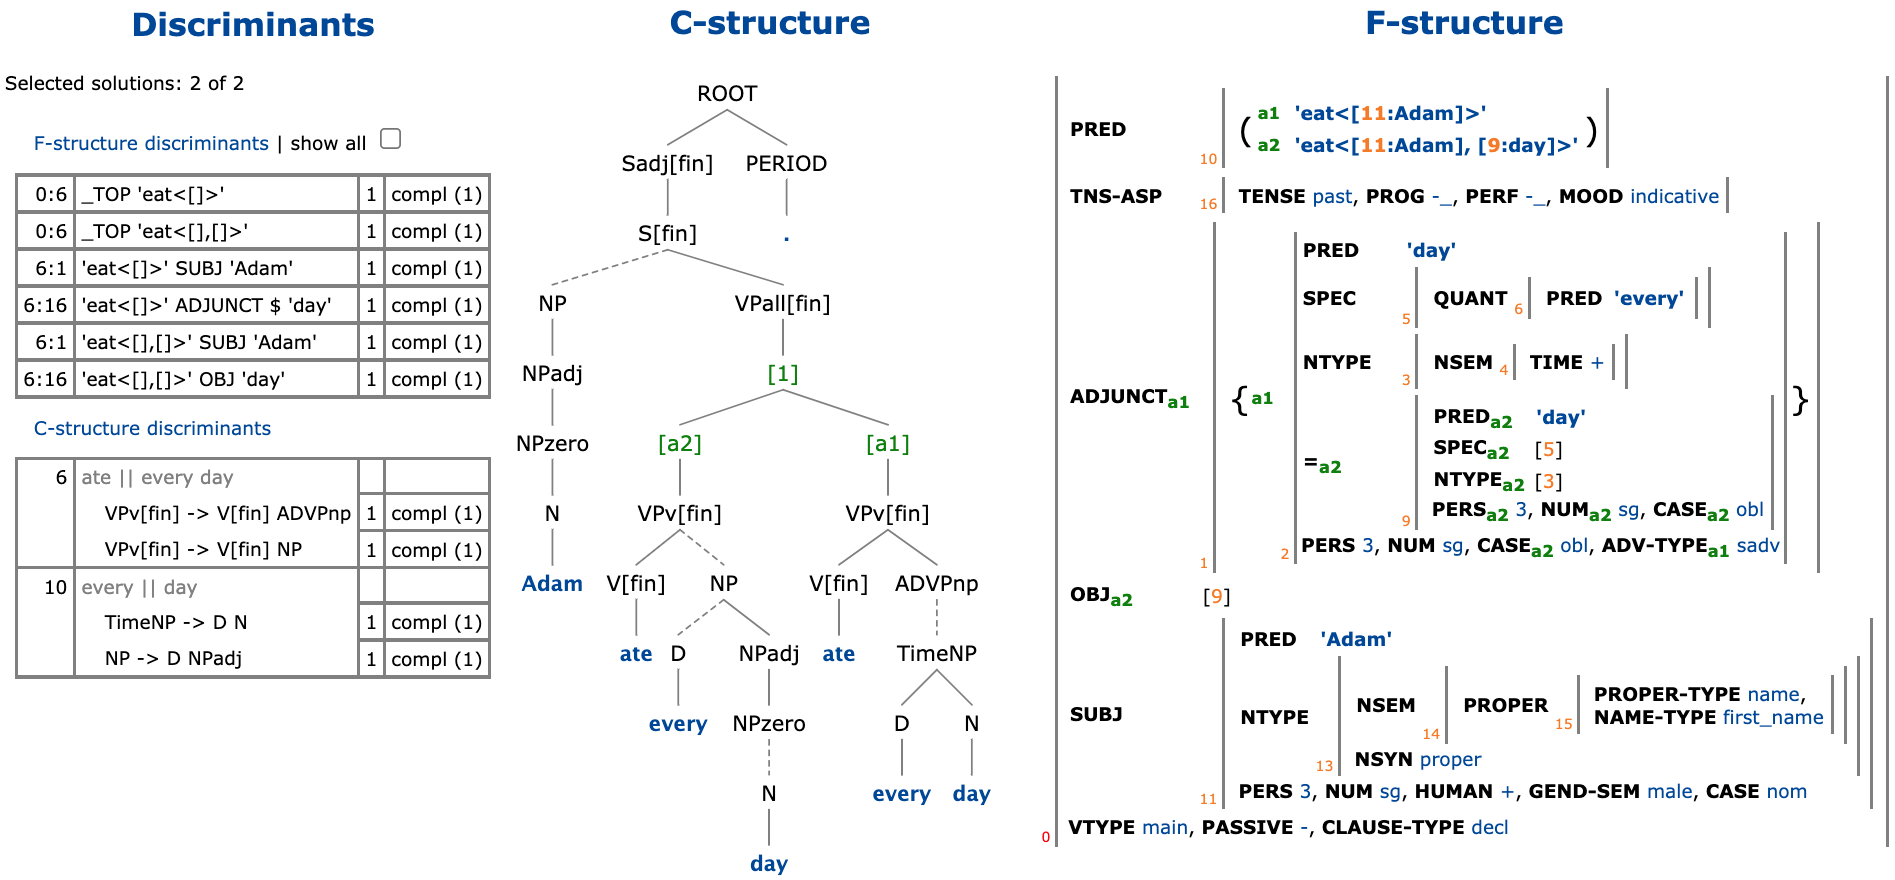
\includegraphics[width=\textwidth]{figures/Treebanks/Adam-expanded.png}
 %   \caption{Analysis with discriminants for %\textit{Adam ate every day.}}
  %  \label{fig:Adam}
%\end{figure}

\begin{figure}
    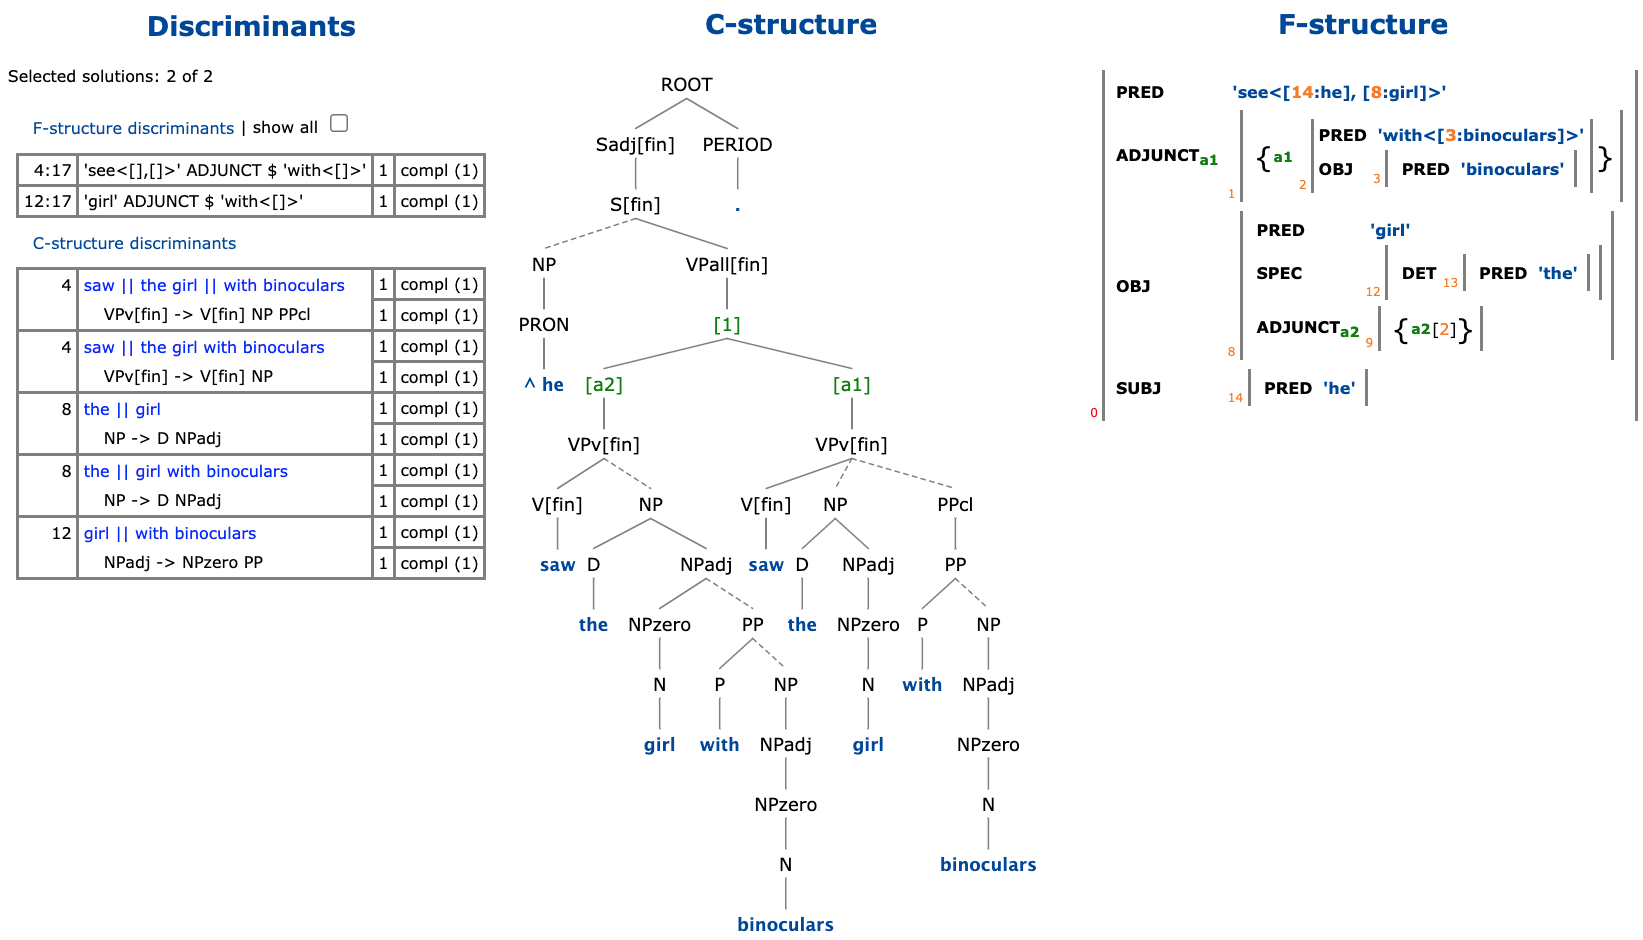
\includegraphics[width=\textwidth]{figures/Treebanks/binoculars.png}
    \caption{Analysis with discriminants and packed c- and f-structures for \textit{He saw the girl with binoculars.}}
    \label{fig:binoculars}
\end{figure}

This sentence has two possible analyses due to a PP attachment ambiguity:  \textit{with binoculars} may be either an \textsc{adjunct} of the clause or an \textsc{adjunct} in the \OBJ.
%There are three analyses for this sentence due to interconnected lexical and syntactic ambiguities: in one analysis the word \textit{can} is a modal auxiliary which takes an \XCOMP headed by the main verb \textit{fish}; in the other two analyses the word \textit{can} is a transitive verb which takes an \OBJ, with \textit{fish} being either a singular or plural noun.
%There are two analyses for this sentence, one where the phrase \textit{every day} functions as the \OBJ, and one where it functions as the \textsc{adjunct}.
Whereas XLE offers packed f-structures, XLE-Web offers packed representations for both c- and f-structures.
A packed representation presents all analyses in one graph, with indices at choice points.
In the middle of \figref{fig:binoculars} is a packed c-structure with one choice point which splits into the subtrees labeled \emph{a1} and \emph{a2}.
A corresponding choice can be seen in the packed f-structure shown on the right in the figure.
%In the f-structure, various attributes and values are also labeled with \textit{a1} and \textit{a2} depending on which of the subtrees they are projected from.
Although the disambiguated f-structure will have an \textsc{adjunct} either on the outer level or inside the \OBJ, both functions occur in the packed f-structure, labeled with \textit{a1} and \textit{a2} respectively.
%Parentheses indicate alternative values for the attributes \textsc{pred}, \textsc{vtype} and \textsc{num}.


%The parentheses encompassing \textit{a1} and \textit{a2} in the value of the \textsc{pred} of the outer f-structure indicate that the semantic form has either a one-place predicate taking only a \SUBJ or a two-place predicate taking a \SUBJ and an \OBJ.
%This difference in semantic forms is correlated with the difference in how the phrase \textit{every day} is represented in the f-structure.
%When \textit{eat} is a one-place predicate, the phrase \textit{every day} is the \textsc{adjunct}; when \textit{eat} is a two-place predicate, the phrase \textit{every day} is the \OBJ.

%This f-structure is displayed in \emph{\textsc{pred}s only} mode, an abbreviated f-structure display which may be used for instance when the full f-structure is too large to fit on the screen, or, as here, too large to be legible in a figure.
%in which some features are hidden from view for the sake of clarity.

On the left in the figure is a table with discriminants computed on the basis of these choice points.
They present the user with each individual distinction between the analyses.
There are two f-structure discriminants and ten c-structure discriminants.\footnote{In some cases there may also be lexical and morphological discriminants, but not for this sentence, which does not display any lexical ambiguities.}
F-structure discriminants describe paths through the f-structure from a \textsc{pred} value to another \textsc{pred} value or an atomic value.
The two f-structure discriminants shown here indicate that the phrase \textit{with binoculars} is an \textsc{adjunct} either of the verb \textit{see} or of the noun \textit{girl}.
The ten c-structure discriminants present the various minimal subtrees (a minimal subtree being a mother node and its daughter nodes) that make up the subtrees indexed with \textit{a1} and \textit{a2}.
C-structure discriminants are either constituent discriminants, which show the bracketing of a substring, or rule discriminants, which show the labeled bracketing of a substring, expressed as a phrase structure rule.
Rule discriminants are always displayed directly under the corresponding constituent discriminant, thus showing clearly which string of words the rule represents a bracketing of.

A discriminant may be chosen by clicking on it, or rejected by clicking on \textit{compl} (for \textit{complement}).\footnote{The numbers to the left of the discriminants are anchors, which are necessary in case the same word or phrase occurs more than once in the sentence.
In c-structure discriminants the anchor identifies the position of the first character in the substring.
In f-structure discriminants the anchors identify the position of the first character of the words that project the \textsc{pred} values in the discriminant.
The number to the right of a discriminant (or its complement) indicates the number of solutions that will remain after the discriminant (or its complement) is chosen.}
%In this case we see that there are several f-structure discriminants (only some of which are displayed---the box \textit{show all} may be ticked to see all f-structure discriminants) and several c-structure discriminants.
After a discriminant or its complement has been clicked on, it is displayed in boldface; the choice may be reversed by clicking on the boldfaced discriminant, thus resetting it.
Since there are only two analyses for the sentence in \figref{fig:binoculars}, the intended one may be selected by choosing or rejecting any one discriminant.
\figref{fig:binoculars-disambiguated} shows the effect of choosing the analysis in which \textit{with binoculars} is an adjunct of the verb \textit{see} by clicking on the first f-structure discriminant, resulting in full disambiguation.
Discriminants that have not been chosen and that are no longer relevant for disambiguation, because they do not distinguish between any remaining analyses, are not displayed.
This is important for efficiency, since the disambiguator then has fewer discriminants to take into consideration.

\begin{figure}
    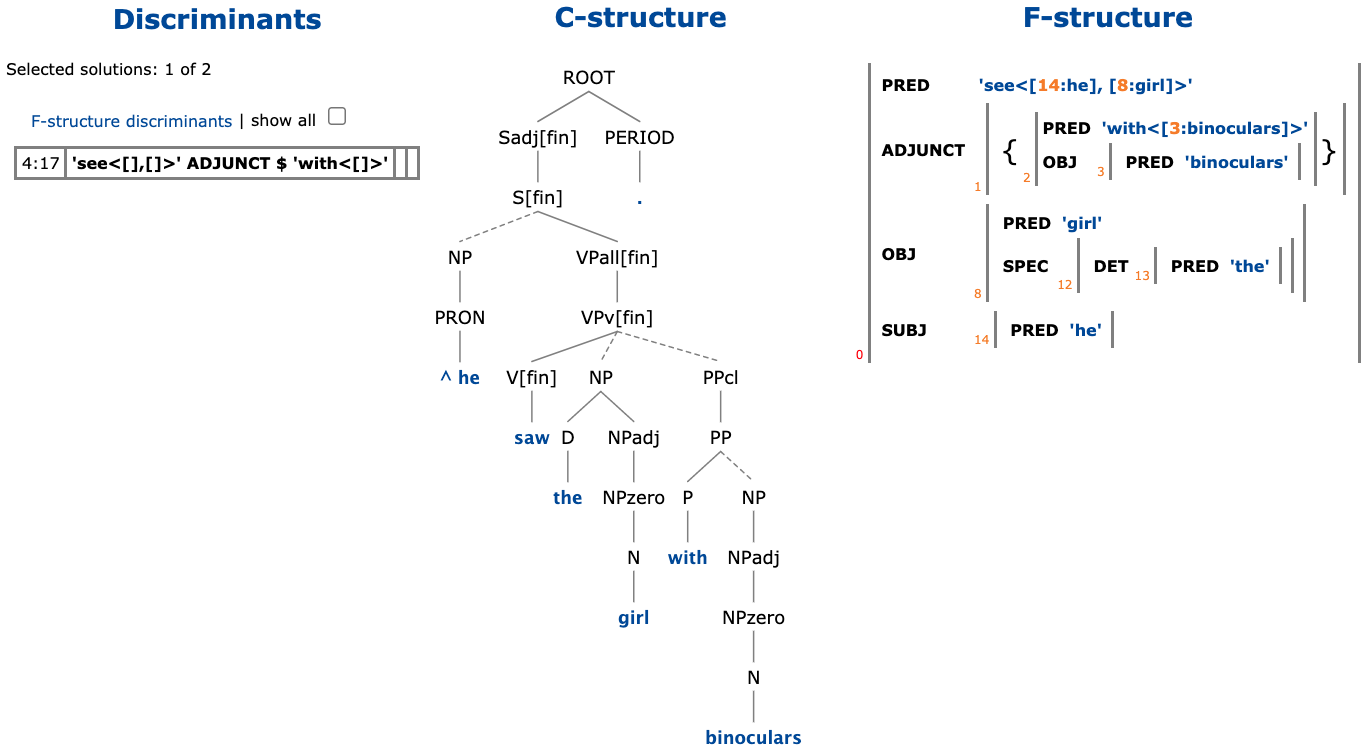
\includegraphics[width=\textwidth]{figures/Treebanks/binoculars-disamb.png}
    \caption{Fully disambiguated analysis for \textit{He saw the girl with binoculars.}}
    \label{fig:binoculars-disambiguated}
\end{figure}

This process may seem like overkill for this simple example which has only two readings. %KDS
It becomes rewarding, however, when there are multiple ambiguities in the sentence. %KDS
Even when the combination of ambiguities may give rise to a very large number of analyses, the number of discriminants does not necessarily increase as much, so that discriminant analysis remains comparatively efficient.
A more detailed presentation of disambiguation with discriminants in LFG may be found in \citet{Rosen07lfg}.%\citet{Meurer}

At the time of writing, the XLE-Web instance at INESS offers online parsing with the ParGram grammars of the following languages: English, French, Georgian, German, Indonesian, Italian, Malagasy, Norwegian, Polish, Tamil, Tigrinya, Turkish, Urdu and Wolof.
Some of these have broad coverage, while others are more limited in scope.

\subsection{The LFG Parsebanker}\label{parsebanker}

The LFG Parsebanker, available in INESS, is an integrated set of tools for creating and searching LFG treebanks \citep{Rosen09}. %KDS
It allows texts to be batch parsed with the XLE parser, and it stores the analyses in a database. %KDS
The resulting parsebank may be disambiguated by using discriminants in the same way as described above.
The LFG Parsebanker stores both the analyses and all discriminant choices that were made. %KDS
This means that the grammar and lexicon may be further developed, and the treebank subsequently reparsed and at least partially redisambiguated with the stored discriminant choices.
This method makes it possible to develop the grammar and the treebank in tandem, thus incrementally improving the quality of the analyses.
The stored discriminants may also be used for stochastic parseranking.
In this way larger parsebanks can be automatically disambiguated.

A possible drawback of constructing a treebank by parsing with an LFG (or other) broad-coverage unification grammar is that the grammar cannot hope to have full coverage for all authentically occurring sentences in a large corpus.
Nevertheless, some traditional treebanks that are (at least partially) manually annotated are meant to assign an analysis to every sentence, and a variety of methods are utilized to achieve this.
When a sentence is not covered by the grammar, an annotator can, for instance, manually construct an analysis to ``fix'' the problem.
Although this provides an analysis for the treebank, it does not provide an analysis that is consistent with a grammar, and sentences that are not actually grammatical may receive analyses as if they were.
In contrast, a pure parsebank does not resort to such ad hoc fixes, since it is often primarily meant to test the coverage and precision of a grammar, so that it is desirable to keep the treebank in sync with the grammar.
The LFG Parsebanker therefore does not permit disambiguators to edit the automatically derived analyses, but allows them to make notes for grammar and lexicon development to solve coverage problems.

\section{LFG treebanks in INESS}\label{iness-treebanks}

INESS is a treebanking infrastructure for building, hosting and exploring treebanks.
It includes the above-mentioned XLE-Web and the LFG Parsebanker.
It also has an elaborate infrastructure for browsing, search and visualization, as will be explained below.

INESS accommodates not only LFG treebanks, but also treebanks based on other frameworks, such as HPSG \citep{pollard1994head-driven}, constituency, and dependency treebanks.
The infrastructure makes treebanks available online in an internet browser, eliminating the need to download treebanks and software for viewing and searching them, thus considerably facilitating access to them.
Since INESS hosts many treebanks, there is an interface for treebank selection, as described in \sectref{select}.

While some treebanks have completely open access, others require user authentication and authorization.
Treebank owners decide under what licensing terms their treebanks are to be made available; some treebanks have restrictive licenses due to copyright of the input texts.
The most open license that copyright will allow is recommended \citep{Rosen21Managing}.
INESS participates in the CLARIN Service Provider Federation (SPF), which allows researchers to authenticate themselves by logging in with their own university credentials, thus gaining access to many more treebanks than are freely available.
The CLARIN SPF has participant institutions in many countries, both in Europe and beyond.
Users not belonging to one of these institutions can apply for a user name and password at CLARIN.\footnote{CLARIN is a digital infrastructure offering data, tools and services to support research based on language resources (\url{http://clarin.eu}).}

INESS hosts LFG treebanks of varying sizes.
The larger treebanks TIGER, the LFG Structure Bank for Polish, and NorGramBank are presented in \sectref{tiger}, \sectref{polfie} and \sectref{norgrambank}, respectively.
The smaller treebanks are presented in \sectref{small}.
INESS also hosts several parallel treebanks with LFG annotations, presented in \sectref{parallel}.
%The exploration of LFG treebanks will be presented in \ref{inessearch}.
The INESS interface is described in more detail by \citet{Meurer20Interactive}. %KDS

\subsection{Selecting treebanks in INESS}\label{select}

The first step in exploring treebanks involves selecting one or more treebanks.
%\note{This could be one or more as in a parallel treebank, or it could be one or more as in comparing UD treebanks wrt annotation consistency.}
At the time of writing, INESS hosts 433\footnote{According to \figref{fig:choice}, there are 1057 treebanks in total, but this number includes all of the versions of the UD treebanks. If we only count the number of treebanks in Universal Dependencies 2.5 (200), the total number of treebanks is 433.} treebanks for 115\footnote{There are 117 language names, but three of these are Norwegian, Norwegian Bokmål, and Norwegian Nynorsk, and these have been counted as one language: Norwegian. Norwegian Bokmål and Norwegian Nynorsk are the two written standards for the Norwegian language, with a good deal of lexical variation and many differences in spelling and morphology. Most treebank texts are written consistently in one variety or the other, so that users can choose which written variety to explore. Some texts, however, contain both varieties, for instance the proceedings of the Norwegian parliament `Stortinget'; the latter are categorized simply as Norwegian.} languages.
The \emph{Treebank Selection} page in INESS, shown in \figref{fig:choice}, groups treebanks according to language, collection and type.

\begin{figure}
    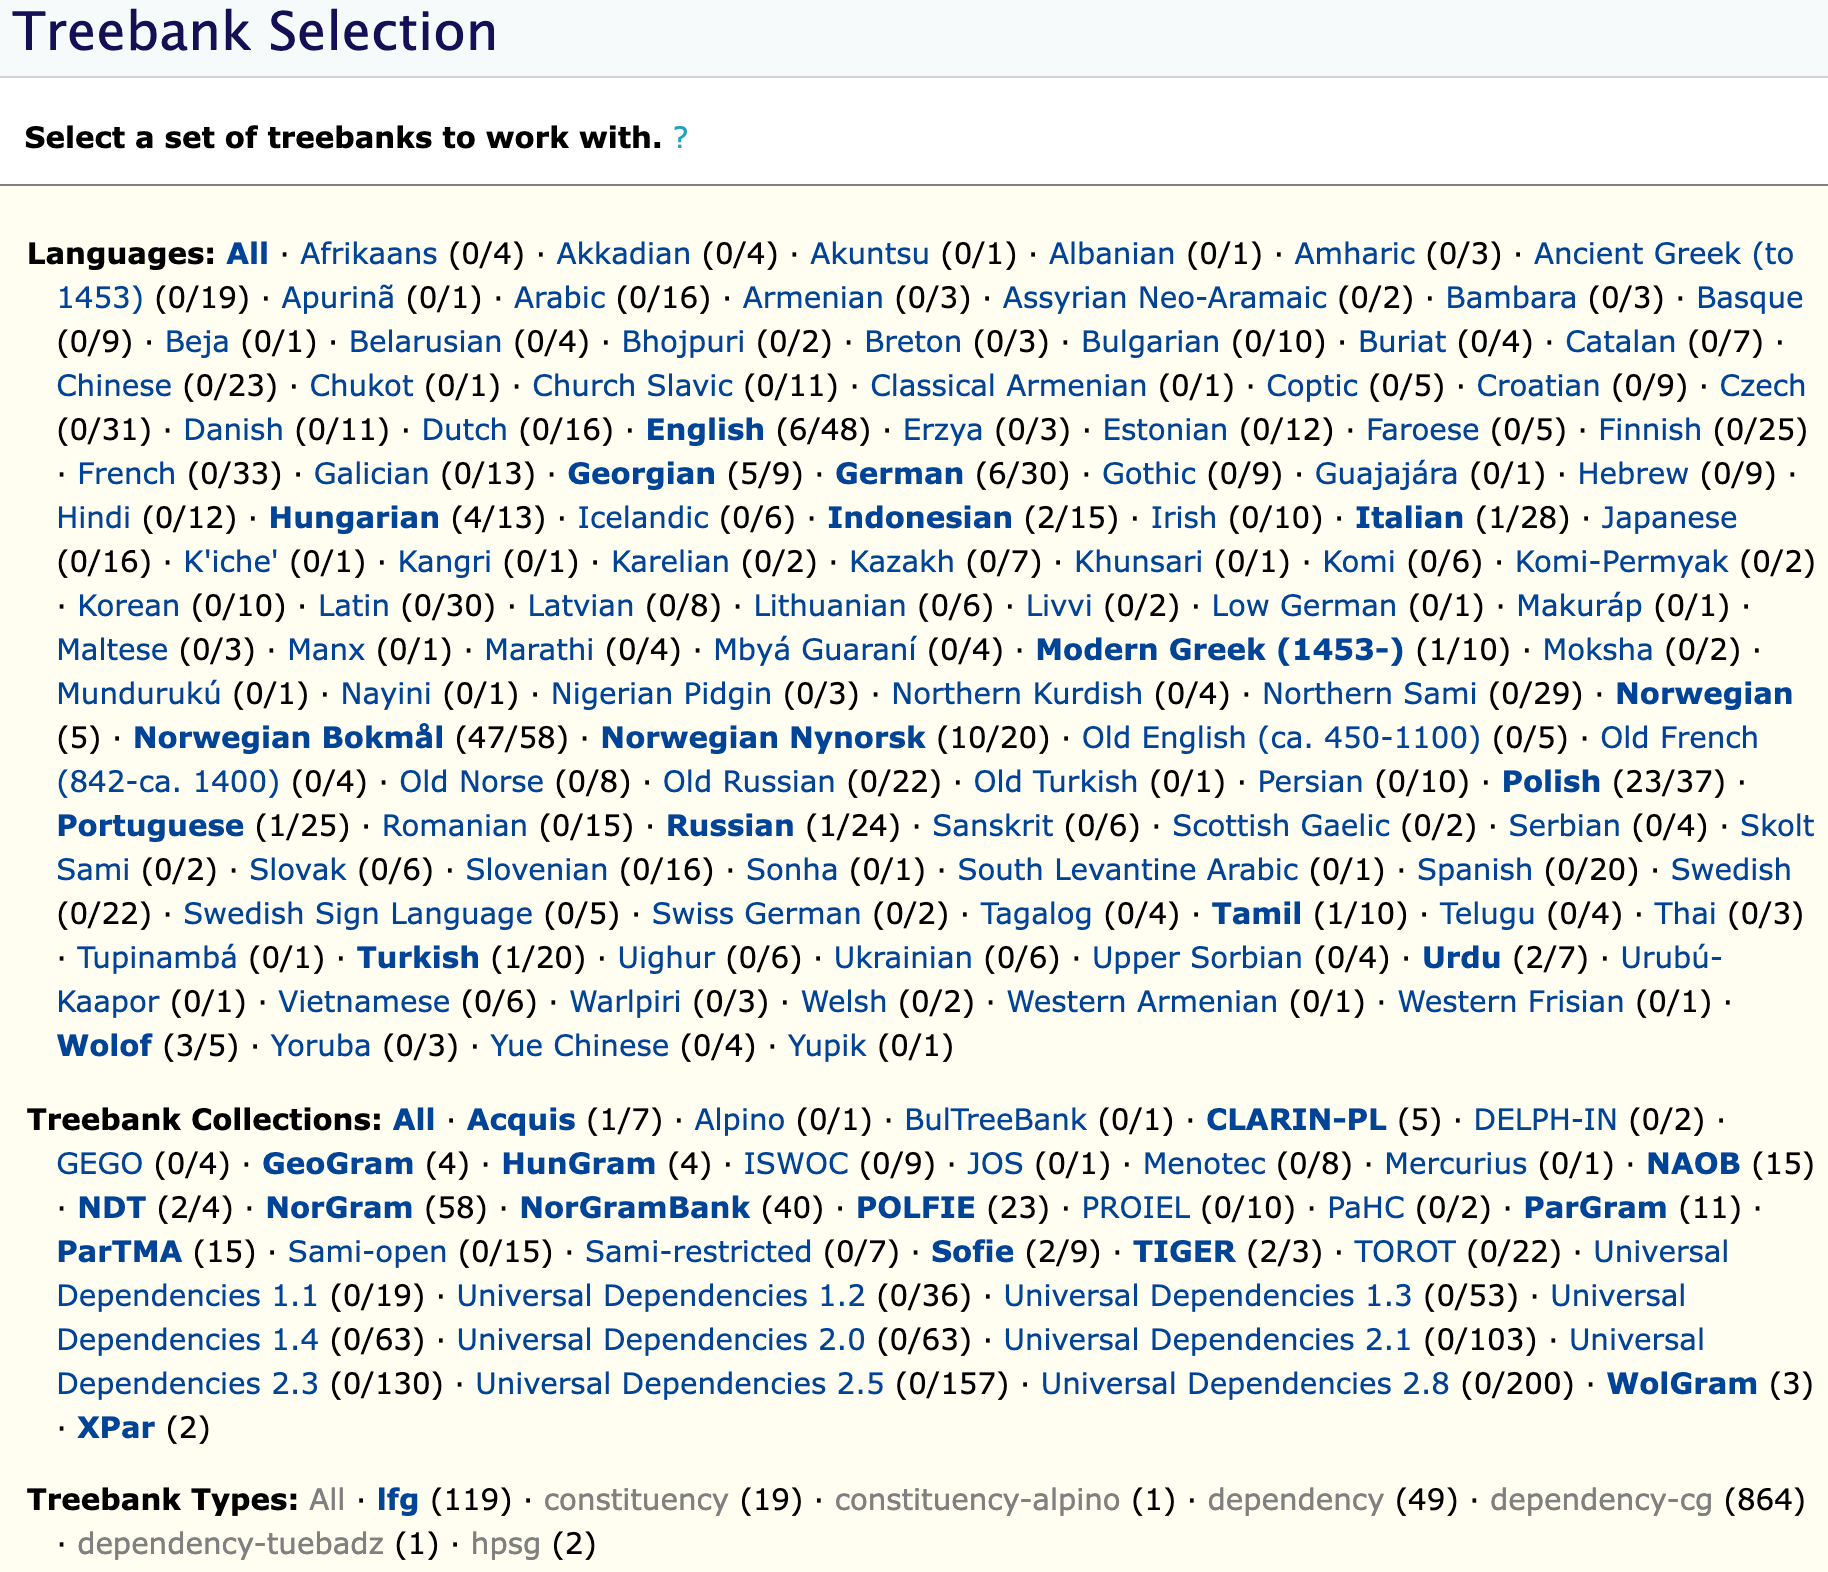
\includegraphics[width=\textwidth]{figures/Treebanks/LFG-choice-3.png}
    \caption{The INESS user interface for treebank selection, with treebank type \textit{lfg} chosen}
    \label{fig:choice}
\end{figure}

A collection contains several treebanks with something in common, for instance that they were developed as part of a specific project, or that they consist of translations of the same text into different languages (including the source language text).
A single treebank may belong to more than one collection.
Type refers to the annotation type, such as LFG, HPSG, constituency, and dependency, and includes subtypes of these.
The user may click on any language, collection or type to make a first choice about which treebanks should be displayed.

In \figref{fig:choice} we see the effect of clicking on the type \textit{lfg}; after this choice, only the languages and treebank collections that have LFG treebanks are displayed in boldface.
Counting the boldfaced languages in \figref{fig:choice} shows that there are 16 languages that have LFG treebanks.
After each language name, the numbers in parentheses indicate how many of the treebanks are LFG treebanks; for English, (6/48) means that six of 48 treebanks are LFG treebanks.
In a similar manner, under Treebank Collections, TIGER (2/3) means that two of the three treebanks in the collection called TIGER are LFG treebanks. %KDS: In Figure 4, there are three TiGer treebanks which are LFG treebanks, not two.

Once a first choice has been made by a user, a list of all treebanks matching that choice is displayed.
When LFG is chosen, a total of 119 treebanks are listed.
The top of this list is shown in \figref{fig:top}.\footnote{
Treebank names in INESS begin with the three-letter ISO 639-3 code for the relevant language.}
For each treebank, this overview shows its name, which collections it belongs to, its annotation type, its size (in sentences and words), whether it has been indexed for search, and the type of license (if any).
The user may choose one or more treebanks by ticking off the boxes to the left of the treebank name; 
clicking on the name of one of the chosen treebanks brings the user to that treebank.
When exploring a treebank for the first time, the user is asked to accept the license conditions.

Clicking on a treebank name brings the user to the \emph{Sentence Overview} page for that treebank; the sentences are listed one per line together with information about their disambiguation status.
Clicking on a sentence displays the \emph{Sentence} page, where the analysis for that sentence is shown including the textual context the sentence occurs in (the previous and following three sentences).

\begin{figure}
    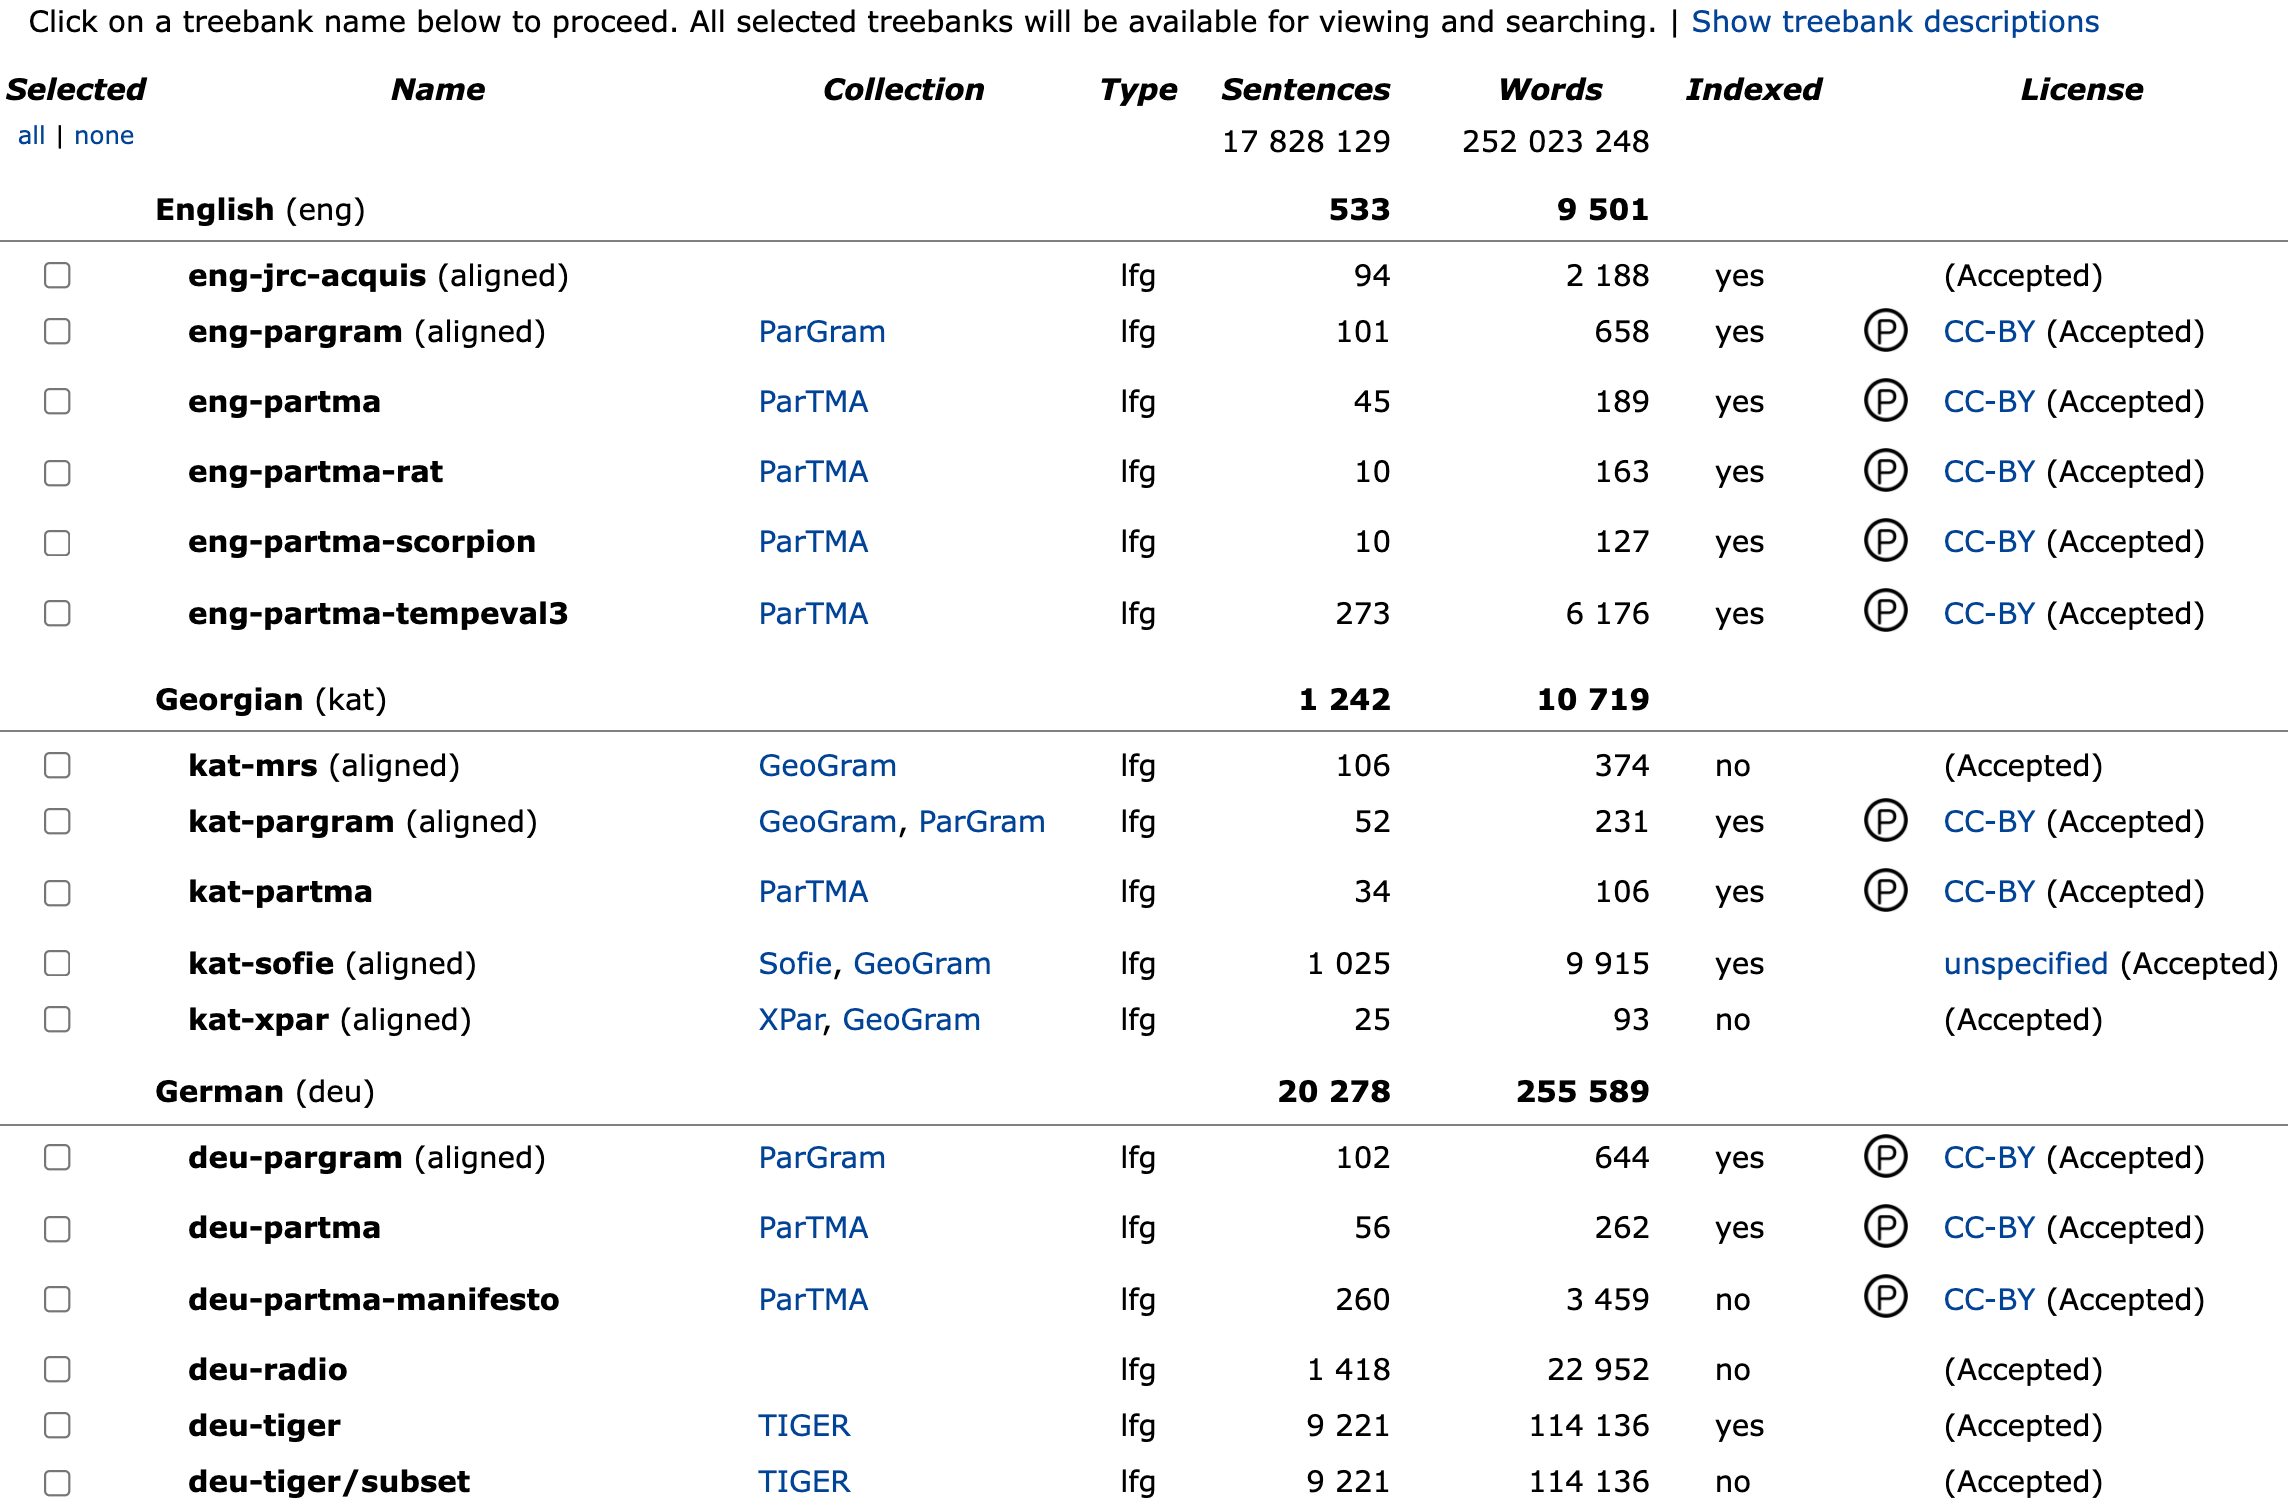
\includegraphics[width=\textwidth]{figures/Treebanks/top-new-5.png}
    \caption{Top of the list of treebanks after the  type \textit{lfg} has been chosen}
    \label{fig:top}
\end{figure}


\subsection{The TIGER treebank}\label{tiger} % KDS: should this be written as TiGer passim, as in Figures 3 and 4?

%The original TIGER treebank of German newspaper text \citep{Lezius02,Brants02tlt,brants2004} is a hybrid between constituency and dependency annotation; part of it is also annotated with LFG structures.
The original TIGER treebank of German newspaper text \citep{Brants02tlt,brants2004} uses a hybrid annotation combining constituency and dependency information; part of it is also annotated with LFG structures.
The constituency/dependency part of the treebank was constructed by two different methods.
In one method a cascaded probabilistic parser was used in combination with manual annotation with the ANNOTATE tool \citep{Brants00}.
The other method involved parsing with the German LFG grammar, followed by manual disambiguation; the XLE transfer system was employed to change the representations into the TIGER format \citep{zinsmeisteretal02}.
The LFG analyses were thus originally utilized in an experimental way to construct a more traditional treebank, but they now also constitute a useful resource as a standalone LFG treebank.
%The LFG analyses were thus not originally meant to constitute a treebank on their own, but were just an experimental way of constructing a more traditional constituency treebank.

%A drawback of constructing a treebank by parsing with an LFG (or other) broad-coverage unification grammar is that the grammar can never have full coverage for all authentically occurring sentences in a text.
%Traditional treebanks are meant to cover all sentences, and a variety of methods are utilized to achieve this.
%When a sentence is not covered by the grammar, an annotator can hand construct an analysis to ``fix'' the problem.
%Although this provides an analysis for the treebank, it does not provide an analysis that is consistent with the grammar.
%And it sometimes means that sentences that are not actually grammatical will receive analyses as if they were.

%The advantage of constructing a treebank by parsing with a wide-coverage grammar is that the grammar will always be in sync with the treebank.
%Not all sentences in a corpus will be covered, but the sentences that are covered will have more well-founded analyses.

%The LFG analyses that were used for creating (part of) the TIGER treebank are made available as a standalone treebank in INESS.
%They constitute an interesting treebank resource in their own right.

\figsref{fig:davon-tiger}{fig:davon-tigerLFG} display the constituency/dependency and LFG analyses, respectively, for the sentence in (\ref{ex:davon}). The URLs in parentheses in the captions are PIDs (persistent identifiers). They provide links to the analyses in the treebanks. Such links are persistent as long as the treebank they refer to remains available. For treebanks with certain licensing conditions, the PIDs may only work if the user is logged in and has accepted the license. For LFG treebanks, which are dynamic (they can be reparsed after changes are made to the grammar and/or lexicon), the PIDs are persistent in the sense that they provide a link to the \emph{current} analysis of the sentence in the treebank.

\ea German\\
\gll Das Angebot ist bereits groß.\\  
     the offer is already large\\ 
\glt `The offer is already large.'
\label{ex:davon}
\z

\begin{figure}
    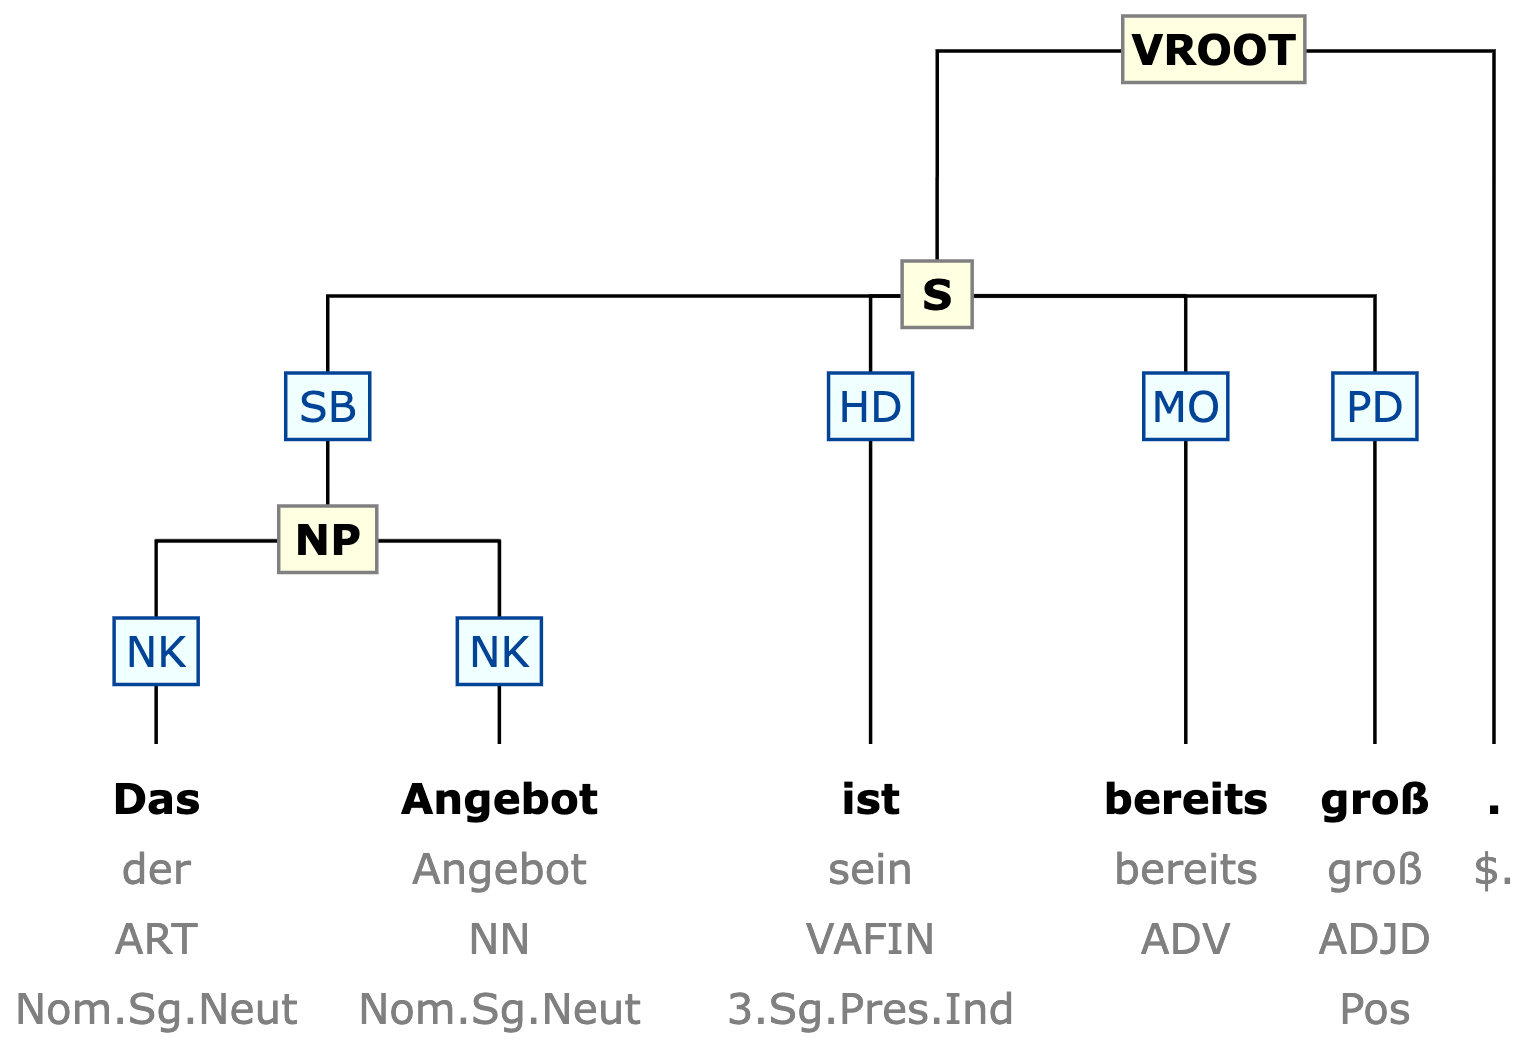
\includegraphics[width=0.55\textwidth]{figures/Treebanks/Angebot-TIGER.png}
    \caption{TIGER constituency/dependency analysis of
      (\ref{ex:davon}) (\url{http://hdl.handle.net/11495/D8B8-3970-851A-3@dep138682})}
    \label{fig:davon-tiger}
\end{figure}

\begin{figure}
    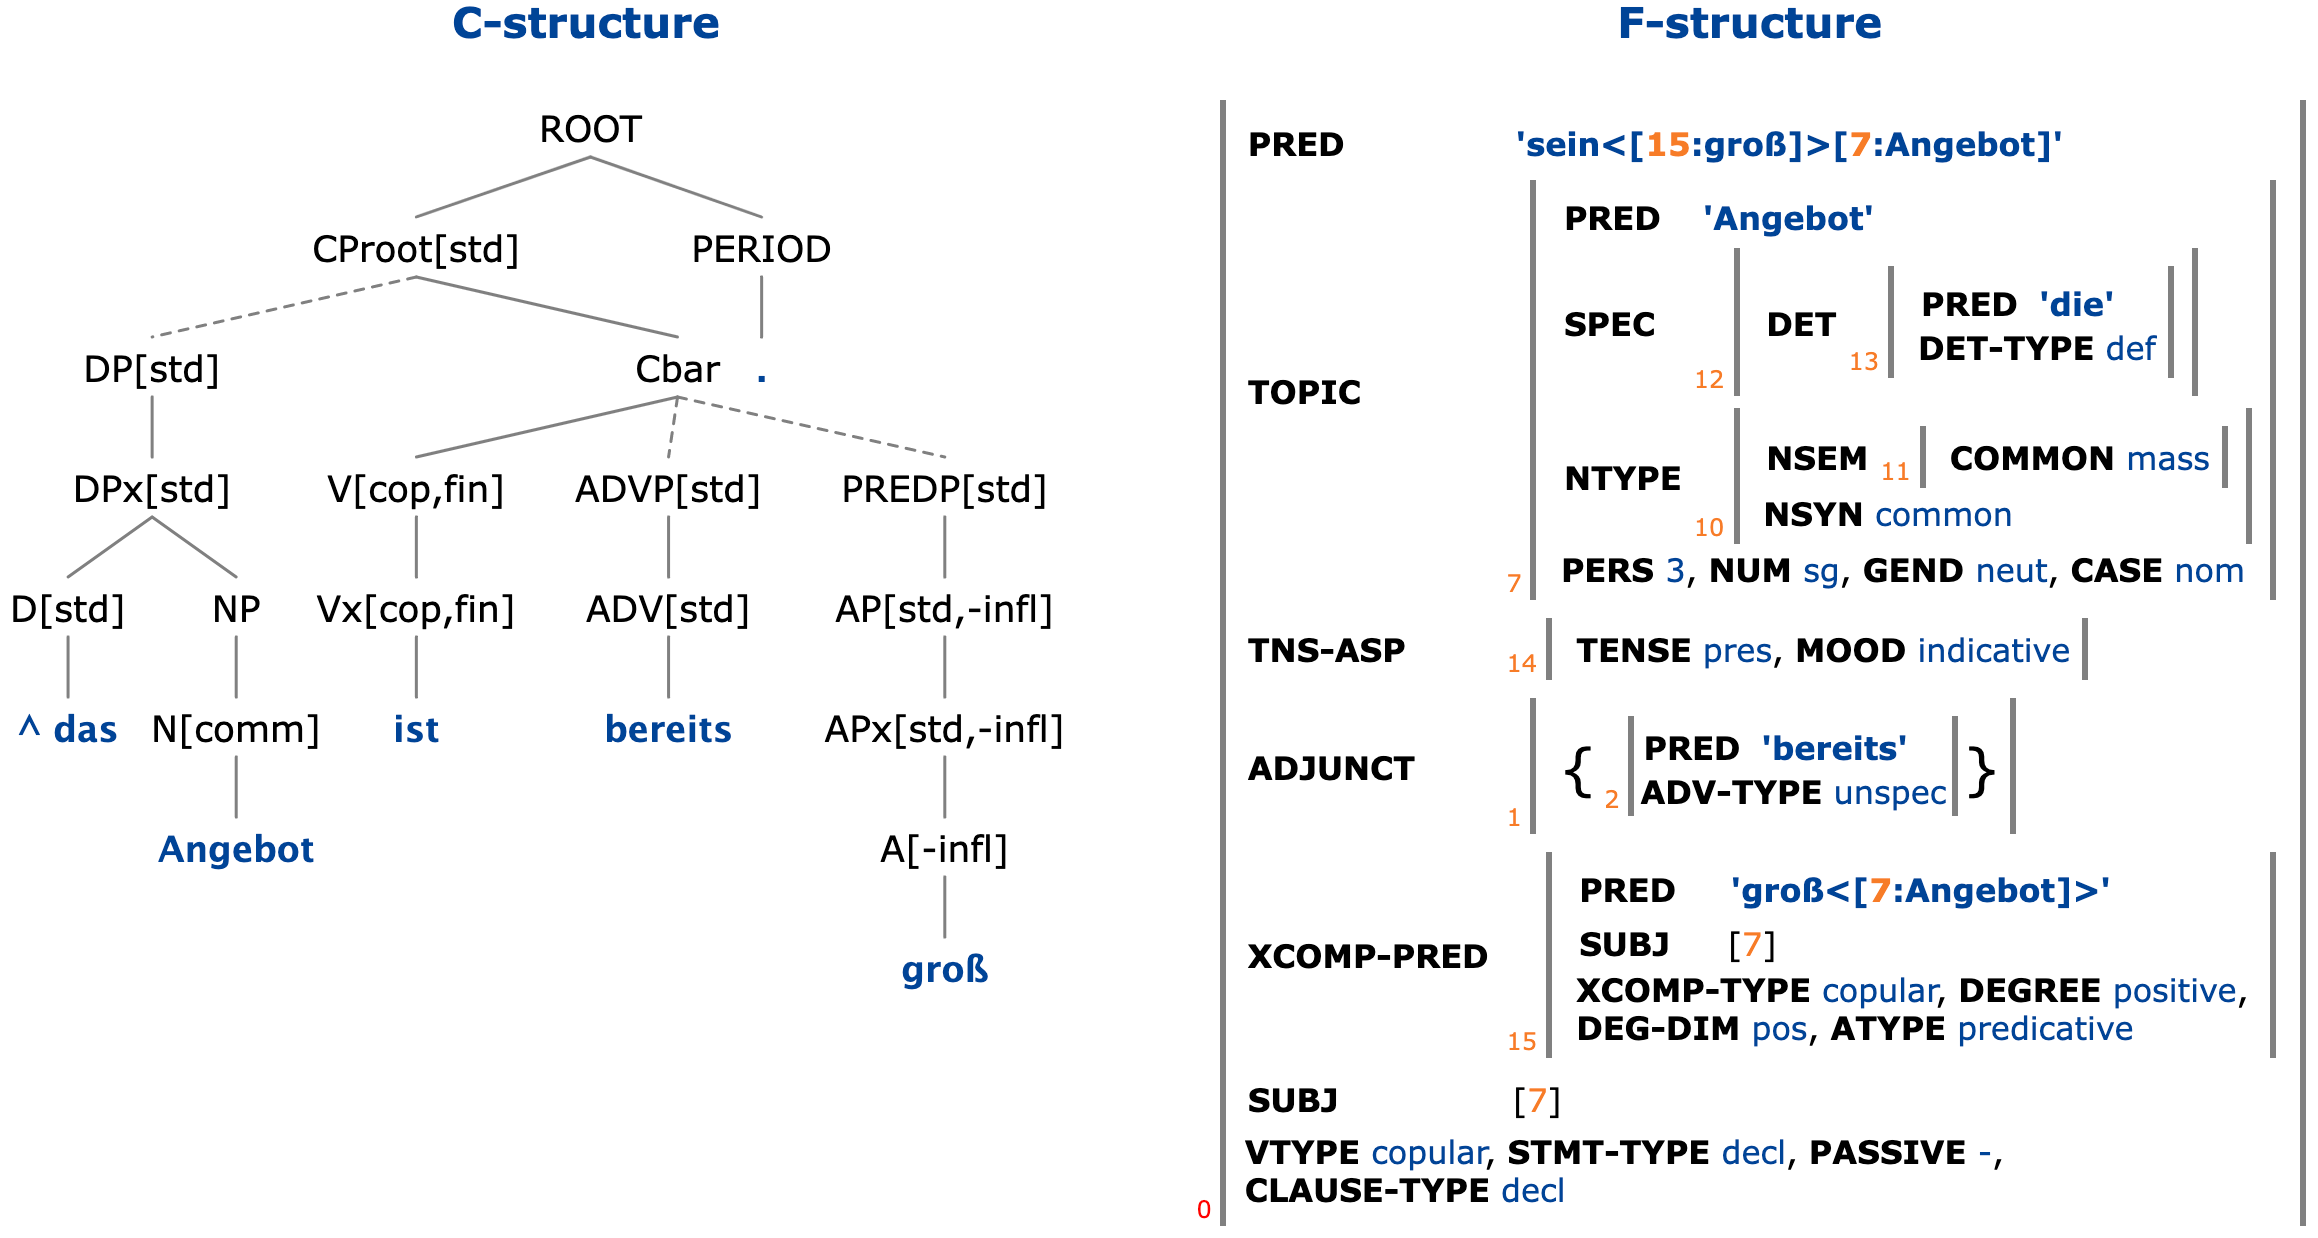
\includegraphics[width=\textwidth]{figures/Treebanks/Angebot-LFG.png}
    \caption{TIGER LFG analysis of (\ref{ex:davon}) (\url{http://hdl.handle.net/11495/D8B8-3970-851A-3@lfg41730})}
    \label{fig:davon-tigerLFG}
\end{figure}

The tree in \figref{fig:davon-tiger} contains information about both phrase structure and syntactic functions.
The nodes in yellow boxes are phrasal categories, while the nodes in the blue boxes under the S node are syntactic functions: %KDS: if this is a citation, add reference
\textsc{sb} for subject, \textsc{hd} for head, \textsc{mo} for modifier and \textsc{pd} for predicate complement.

The c-structure in \figref{fig:davon-tigerLFG} displays extensive unary branching -- many nodes have only single daughters -- and many complex category labels, i.e., c-structure nodes subscripted with features enclosed in square brackets.
The latter device moves some of the feature complexity of the LFG grammar from the f-structure space into the context-free c-structure space, which improves parsing efficiency while maintaining the simplicity of the c-structure rules.
In the f-structure we see that the \SUBJ is also analyzed as the \textsc{topic}, the predicate complement is analyzed as an \textsc{xcomp-pred}, and the modifier is analyzed as an \textsc{adjunct}.

%Size: 18,505 sentences, 229,252 words

%From the metadata for the collection The TIGER treebank (TIGER): The TIGER collection consists of two treebanks:

%The original TIGER Treebank (Version 2.1), annotated as a constituency treebank with crossing branches and secondary edges.
%It consists of app. 900,000 tokens (50,000 sentences) of German newspaper text, taken from the Frankfurter Rundschau. The corpus was semi-automatically POS-tagged and annotated with syntactic structure.
%Moreover, it contains morphological and lemma information for terminal nodes

%The LFG version of the TIGER treebank. (More info!)


\subsection{The LFG Structure Bank for Polish}\label{polfie}

The LFG Structure Bank for Polish was built by parsing a corpus with the POLFIE grammar \citep{patprz12,patprz14}.
This grammar was created by reusing context-free grammar rules written for another parser for Polish, Świgra, and adding annotations for building the f-structures.
The corpus for the treebank is the one-million word subcorpus of the National Corpus of Polish\footnote{\url{http://nkjp.pl/index.php?page=0&lang=1}} which has been manually annotated, the same subcorpus that was used for the previously annotated Składnica treebank.\footnote{\url{http://zil.ipipan.waw.pl/Składnica}} 

In INESS, the treebanks created by the POLFIE grammar are all in one large collection, also called POLFIE.
This collection includes the LFG Structure Bank for Polish as well as other treebanks.
The size of the POLFIE collection is 179,994 sentences and 2,022,026 words.
Some of the subtreebanks in POLFIE are also in other collections: CLARIN-PL, ParGram and ParTMA.

Sample c- and f-structures from the POLFIE treebank for the sentence in (\ref{ex:yesterday}) are given in \figref{fig:Polish-cf}.%\footnote{The PID for this sentence is \url{http://hdl.handle.net/11495/D8B8-3970-851A-3@lfg1411740.}}

\ea Polish\\
\gll Drzewo zostało ścięte wczoraj.\\
     {tree.\NOM.\SG.\N}  get.\textsc{3sg.\N} {cut.\NOM.\SG.\N} yesterday\\ 
\glt `The tree was cut down yesterday.'
\label{ex:yesterday}
\z

\begin{figure}
    \includegraphics[width=\textwidth]{figures/Treebanks/Polish-cf}
    \caption{C- and f-structures for the Polish sentence in (\ref{ex:yesterday}) (\url{http://hdl.handle.net/11495/D8B8-3970-851A-3@lfg1411740})
    \label{fig:Polish-cf}}
\end{figure}

In the c-structure we see some familiar categories such as A, ADV, ADVP, NP, N, I, Ibar, etc., but there are also categories which we might not immediately be able to identify, such as ILEX, PRAET and PPAS.
Some terms in the f-structure may also be unfamiliar, such as \textsc{ntype}, \textsc{nsem} and \textsc{nsyn}.\footnote{These f-structure attributes also occur in \figref{fig:davon-tigerLFG}, and they illustrate the parallelism on the f-structure level achieved by the ParGram grammars; see \sectref{pargram}.}
Treebank documentation should ideally be made available by treebank creators to assist users in exploring the treebank; unfortunately INESS lacks documentation for many treebanks. %VR Documentation on these labels and how they are used should be made available by treebank creators to assist users in exploring the treebank.%KDS: "should"? Are they available or not?

An overview of all \textit{indexed attributes} for each treebank may be found on the \emph{Treebank Details} page.
The indexed attributes are all labels used in the treebank annotation that can be searched for.
For LFG treebanks, these attributes include \textit{cat} (category) and \textit{edge} (feature or attribute, in more standard LFG terminology). 
A screenshot of the top of this page is shown in \figref{fig:details}.

\begin{figure}
    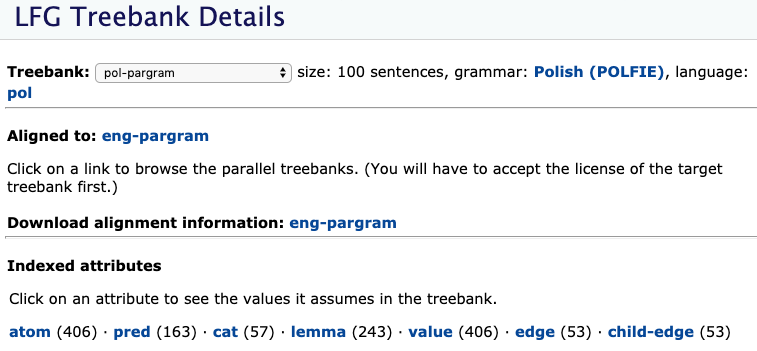
\includegraphics[width=0.9\textwidth]{figures/Treebanks/details}
    \caption{Treebank details for POLFIE}
    \label{fig:details}
\end{figure}

Clicking on \textit{cat} and \textit{edge} under \textit{Indexed attributes} produces the lists in \figref{fig:cat}.
These lists are shown sorted according to frequency; we see that, for instance, the category NP occurs 236 times in this subcorpus (pol-pargram) consisting of 100 sentences. %KDS
%The Treebank Details page provides a complete overview of all categories and features used in the treebank representations, but it does not explain how these are used; treebank documentation should preferably be made available by treebank creators to assist users in exploring the treebank.

\begin{figure}
    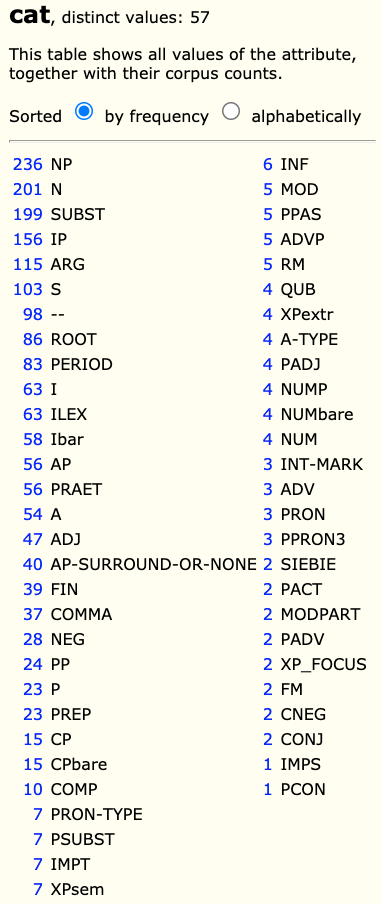
\includegraphics[width=0.43\textwidth]{figures/Treebanks/categories.png}
    \hfill
    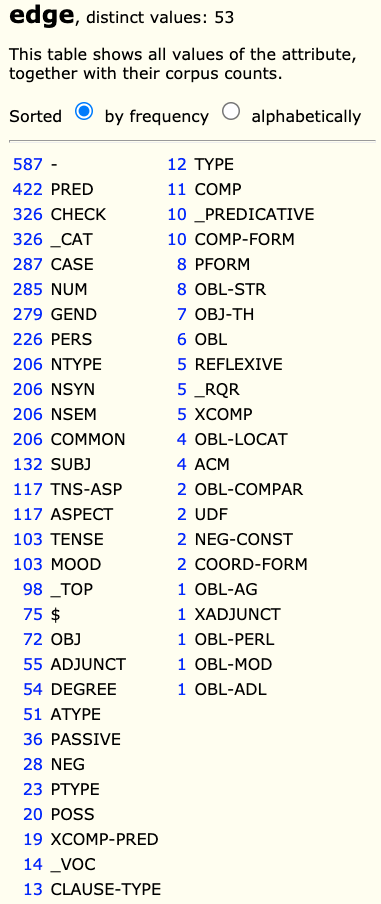
\includegraphics[width=0.43\textwidth]{figures/Treebanks/edges.png}
    \caption{Values for the \textit{cat} and \textit{edge} attributes in POLFIE}
    \label{fig:cat}
\end{figure}

\subsection{NorGramBank: A Norwegian LFG parsebank}\label{norgrambank}

The INESS project had the twofold goal of building a treebanking infrastructure and of building the first large treebank for Norwegian.
%INESS was funded by the Research Council of Norway and the University of Bergen with a total budget of approximately NOK 24 million (around € 2.4 million).
%The project period was from 2010 to 2017.
The result of the latter effort is the treebank collection NorGram, consisting of 15 million sentences (215 million words) and by far the largest LFG treebank available in INESS.
It was parsed with the eponymous grammar NorGram, a wide-coverage LFG grammar developed in the LOGON, TREPIL and INESS projects.
Several versions of this grammar were constructed and used for parsebanking, including versions with c-structure pruning \citep{cahill-etal-2008-speeding}.
Some material was disambiguated manually with discriminants, but the bulk of the parsebank was disambiguated automatically through stochastic parseranking, based on the stored discriminants.

The collection NorGramBank \citep{dyvikEtAl2016} consists of a subset of the texts parsed in the NorGram collection. 
%So the texts in NorGramBank are a subset of those in the NorGram collection.
NorGramBank has more than 160 million words and consists of a variety of text types; while some newspaper texts were included, edited fiction and nonfiction texts were preferred because these have a higher language quality and fewer errors.
Any error in a sentence, whether typographical, orthographical or grammatical, will result in a failure to find the intended analysis on parsing.
Some NorGram texts were excluded from NorGramBank because the source texts had many OCR errors.

\hspace*{-2.5pt}The text selection for the corpus was partially dependent on available resources.
While published texts are valued sources for treebanks and other corpora, copyright restrictions must be taken into account.
It is therefore paramount to clear permissions with rights holders before starting to work on texts.
In the case of NorGram, several texts were obtained through the National Library of Norway.
For some of these, copyright had expired.
For newer texts, exceptional permission to use these with some restrictions was obtained from the government. %KDS
Every corpus must be provided with metadata, including such information as provenance and conditions for use.

The Norwegian treebanks parsed with NorGram have proved useful for lexicography (see \sectref{templates}). 
Some NorGram treebanks have been specifically added for NAOB, a dictionary project by the Norwegian Academy for Language and Literature aimed at building a large dictionary for Norwegian Bokmål.
In INESS, the collection called NAOB consists of 15 treebanks with a total of over 11 million sentences (161 million words). %KDS

The Norwegian example analyses shown in \figsreffive{fig:love-1}{fig:love-2}{fig:skapt-av-gud}{fig:skapt-no-ag}{fig:happy-LFG} are all from the NorGram treebanks.

\subsection{Small treebanks for grammar development}\label{small}

Most of the small LFG treebanks in INESS are test suites used in various projects.
GeoGram, HunGram and WolGram are collections of test suites used for the development of XLE grammars for Georgian \citep{meurer09}, Hungarian \citep{Laczko13,Laczko14} and Wolof \citep{Dione:Disambiguation,Dione19Clause}, respectively.
Some of these test suites are parts of parallel treebanks (see \sectref{parallel}).
Other treebanks in these collections may only be available to their creators since they are work in progress and not at a stage where they may be useful to other researchers.
Treebank developers decide whether they want to make their treebanks publicly available.

%The GeoGram collection 
%
%Size: 1,208 sentences, 10,613 words
%
%This collection contains four LFG treebanks, total words 10613.
%Three of them also belong to other collections (ParGram, Sofie, XPar).
%No metadata for GeoGram itself, only metadata for the other collections it belongs to.

%HunGram

%Size: 3,734 sentences, 17,057 words

%\citep{Laczko14Essentials}

%Wolof

%Size: 2,874 sentences, 40,149 words	
%From metadata for Wolof Treebank testsuite (wol-testsuite): This treebank was used as a testsuite for the Wolof grammar.

%Three treebanks for Wolof.
%In addition to the ParGram test suite, there are two others wol-cwm (460 sentences) and wol-testsuite (2367 sentences).

\subsection{Parallel treebanks with LFG annotations}\label{parallel}

A parallel treebank is a collection of monolingual treebanks that are aligned with each other on the sentence level, and sometimes also on phrase and/or word levels.
The most common type of parallel treebank involves one or more translations of a text that are aligned with the source text, but a parallel treebank can also have different annotations of the same text, for example a constituency annotation and a dependency annotation.

The user can select aligned parallel treebanks by choosing \textit{Show only Parallel Treebanks} on the \emph{Treebank Selection} page and selecting a collection from those that are then displayed in boldface.
One of the treebanks to be examined is then chosen in the usual manner by clicking in the box next to the treebank name and subsequently clicking on the treebank name.
From the \emph{Sentence Overview} page, clicking on \emph{Treebank Details} provides an overview of which other treebanks are aligned.
Selecting one of those treebanks will start the display of parallel analyses for the two chosen languages.

The following subsections will present the XPAR Project (\sectref{xpar}), the treebanks developed in the Parallel Grammar Project (\sectref{pargram}), and other parallel treebanks containing LFG analyses (\sectref{other}).

\subsubsection{The XPAR Project}\label{xpar}

Language Diversity and Parallel Grammars (XPAR) was a pilot project which aimed to determine to what extent the development of parallel deep grammars for typologically diverse languages may support the automatic derivation of high-quality parallel treebanks for those languages \citep{Dyvik09}.
Principles for phrase alignment and methodology for the automatic alignment of c-structures from manually aligned f-structures were developed in the project.

A small parallel test suite of translationally equivalent Georgian and Norwegian sentences was used in developing the alignment tool.
An example of aligned sentences is provided in (\ref{ex:gia}), and their sentence-aligned analyses are shown in \figref{fig:love-1}.

\eal \label{ex:gia}
\ex{Georgian\\
\gll gia-s uqvars eka.\\  
     {Gia-\DAT} loves {Eka.\NOM}\\ 
\glt `Gia loves Eka.'
\ex{Norwegian\\
\gll Jon elsker Maria.\\  
     Jon loves Maria \\ 
\glt `Jon loves Maria.'
}
}
\zl

\begin{figure}
    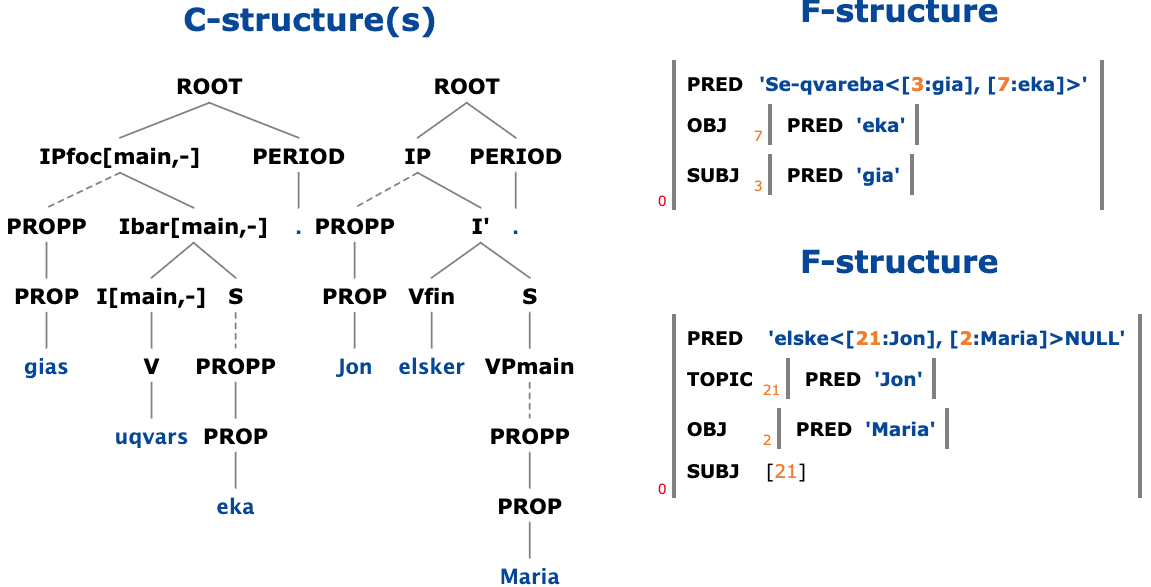
\includegraphics[width=\textwidth]{figures/Treebanks/unaligned}
    \caption{Sentence aligned c- and f-structures for the Georgian (\url{http://hdl.handle.net/11495/D8B8-3970-851A-3@lfg51519}) and Norwegian (\url{http://hdl.handle.net/11495/D8B8-3970-851A-3@lfg60949}) sentences in (\ref{ex:gia})}
    \label{fig:love-1}
\end{figure}

\begin{figure}
    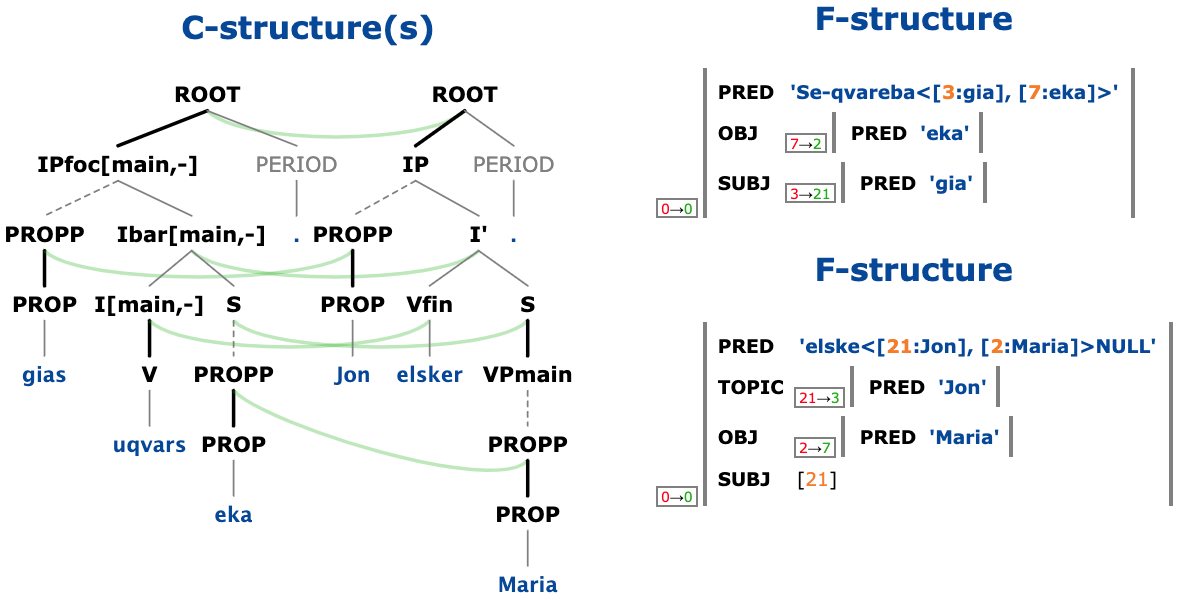
\includegraphics[width=\textwidth]{figures/Treebanks/aligned}
    \caption{Word and phrase aligned c- and f-structures for the Georgian and Norwegian sentences in (\ref{ex:gia})}
    \label{fig:love-2}
\end{figure}

\hspace*{-1.7pt}F-structures are manually aligned on the basis of translational correspondences at the level of predicate--argument structure.
Subsidiary f-structures correspond if their predicates are in a translational relationship to one another.
The alignment is done by dragging the index of one f-structure onto the corresponding index of the other f-structure.
For instance, in \figref{fig:love-1}, the \textsc{obj} index \textcolor{tomato}{$7$} in the Georgian f-structure may be dragged onto the \OBJ index \textcolor{tomato}{$2$} in the Norwegian one.
This results in indices of the form \fbox{{\textcolor{tomato}{$n$}$\rightarrow$\textcolor{kelly}{$m$}}}, where \textcolor{tomato}{$n$} is the original index of that f-structure and \textcolor{kelly}{$m$} is the original index of the f-structure it is aligned with.
\figref{fig:love-2} shows the result of this manual alignment of f-structures, where the indices for the \OBJ, \SUBJ and main \textsc{pred} have been aligned.
Once the f-structures are aligned, the LFG Parsebanker automatically aligns the corresponding nodes in the c-structures, shown by the curved green lines. %KDS
We see, for example, that the \textsc{obj} alignment in the f-structures  results in the alignment of the PROPP nodes dominating \textit{Eka} and \textit{Maria} in the c-structures. 

\subsubsection{The Parallel Grammar Project treebanks}\label{pargram}

The Parallel Grammar Project (ParGram) is an international cooperative effort to develop parallel LFG grammars implemented in XLE \citep{Buttetal:99,Butt02KingMasuichiRohrer}.
Originally three languages were involved in the project: English, French and German; later, other languages joined, including Georgian, Hungarian, Indonesian, Japanese, Norwegian, Polish, Tamil, Turkish, Urdu and Wolof, among others.
The main focus of the ParGram project was to develop and maintain linguistically motivated parallelism at the level of f-structure.
Some of the ParGram participants have also been involved in the ParSem project, an effort to develop semantic structures based on the ParGram syntactic structures, with most of the ParSem systems using XLE’s transfer system.

ParGram has created two parallel treebanks to support the aim of developing parallel LFG grammars.
These treebanks consist of test suites encompassing various syntactic constructions.
The English sentences were first agreed upon, and then translated into the other languages in the project.
The first set of 50 sentences included such constructions as declaratives,  interrogatives, imperatives, transitivity, passive, unaccusative, and subcategorized declaratives \citep{Sulger13acl}.
These sentences are included in the ParGram collection in INESS.
Another set of sentences, concerned with tense, mode and aspect, constitutes the ParTMA collection. \figref{fig:do-support} shows word and phrase aligned c- and f-structures for the English and German sentences in (\ref{ex:farmer}).


\eal \label{ex:farmer}
\ex{What did the farmer see?}
\ex{German\\
\gll Was sah der Bauer?\\  
     what saw the farmer\\ 
\glt `What did the farmer see?'
}
\zl

The f-structures for these sentences are practically identical, whereas the c-structures are quite different.
This is both because the languages are different (English has \textit{do}-support and German does not) and because the grammars for these languages have used quite different principles and techniques in writing the phrase structure rules.
Still we see that most c-structure nodes are aligned.
Since the XPAR principles align only translationally corresponding f-structures with \textsc{pred} values, not all c-structure nodes can be aligned.
The word \textit{did} and the question marks only contribute features to the f-structure, not \textsc{pred} values; these features are not shown here since the f-structures are displayed in \textsc{pred}s only mode.
%The f-structures for these sentences are practically identical, whereas the c-structures are quite different; since the English sentence involves do support, the auxiliary verb is not aligned to anything in the German c-structure.

\begin{figure}
    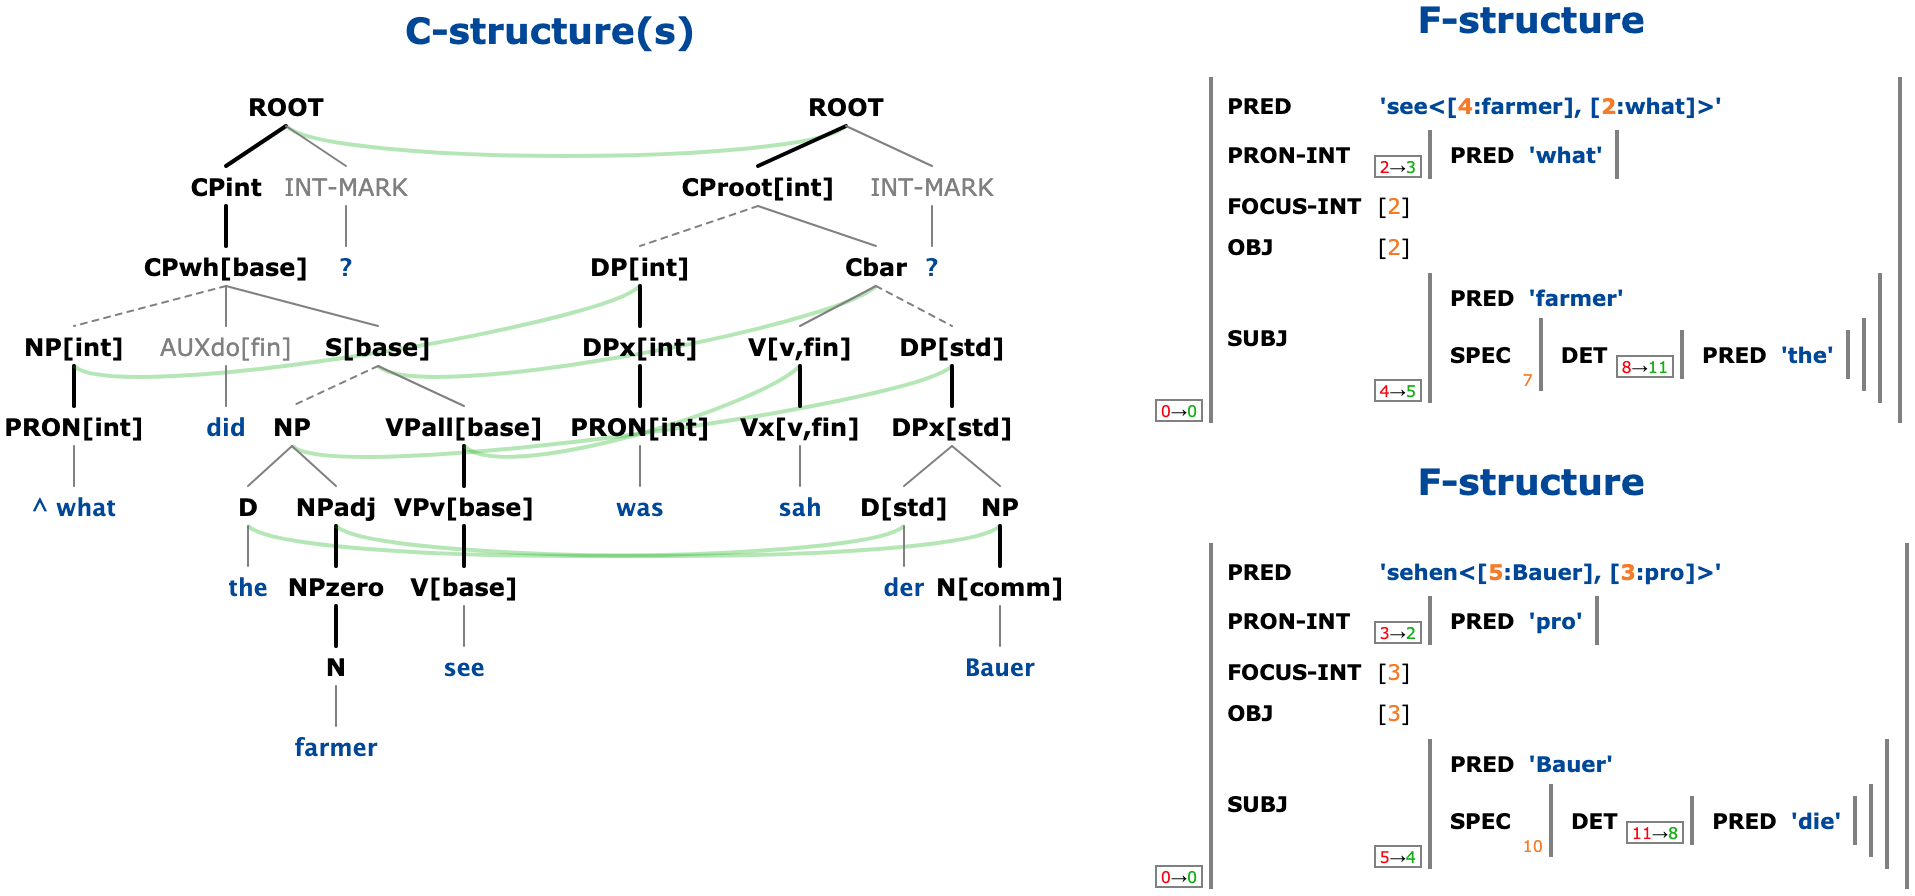
\includegraphics[width=\textwidth]{figures/Treebanks/did.png}
    \caption{Word and phrase aligned c- and f-structures for the English (\url{http://hdl.handle.net/11495/D8B8-3970-851A-3@lfg423651}) and German (\url{http://hdl.handle.net/11495/D8B8-3970-851A-3@lfg444239}) sentences in (\ref{ex:farmer})}
    \label{fig:do-support}
\end{figure}


\subsubsection{Other parallel treebanks including LFG}\label{other} % KDS

Several projects have built parallel treebanks that include both LFG treebanks and treebanks of other types.
Three such parallel treebanks are presented here.

The Sofie Parallel Treebank is a parallel corpus containing the first chapters of Jostein Gaarder's novel \textit{Sofies verden} ``Sophie's World''.
This text was chosen for treebanking because it is a well-written text that has been translated into a great number of languages.
The Nordic Treebank Network developed treebanks based on these texts for Danish, Estonian, German, Icelandic and Swedish in the period 2001–2005.
The META-NORD project,\footnote{\url{http://www.meta-net.eu/projects/meta-nord/}} which ran from 2011 to 2013, had as one of its goals to promote the accessibility of treebanks, including some that had not been maintained and were no longer accessible \citep{Losnegaard13}.
An English treebank, originally developed in the SMULTRON project,\footnote{\url{https://www.ling.su.se/english/nlp/corpora-and-resources/smultron/stockholm-multilingual-treebank-smultron-1.14047
}} and a Georgian treebank, developed at Uni Computing in Bergen, Norway, were added to the Sofie collection.
Two treebanks for Norwegian were also developed, one an LFG treebank and the other a constituency treebank with syntactic and functional categories.
Only the Georgian and one of the Norwegian treebanks have LFG annotation; the rest of the treebanks have various types of constituency annotation.
In the initial version of the LFG Sofie treebank for Norwegian, 73\% of sentences received analyses.
An in-depth study of the sentences that received full parses that were not entirely correct showed that 29\% lacked the correct analysis because of grammar problems, while lexical problems accounted for 71\%, with missing multiword expressions in the lexicon being the most important of these.
Subsequent grammar and lexicon updates resulted in correct analyses for more than 90\% of these sentences \citep{Losnegaard12}. %KDS: you have not defined gold

The META-NORD Acquis Parallel Treebank is a small parallel corpus of translations of a European Union directive.\footnote{Directive 2002/74/EC, from the Acquis Communautaire (AC), the total body of European Union law applicable in the member states.}
The EU languages Danish, Estonian, Finnish, Latvian and Swedish, as well as the non-EU languages Norwegian and Icelandic, have treebanks in the collection.
All language pairs are aligned at sentence level.
The Norwegian treebank contains LFG analyses, while the other languages have consistency or dependency annotations.

The Norwegian Dependency Treebank was developed by the National Library of Norway \citep{Solberg14lrec}; it is made available in INESS as the treebanks named nob-ndt-dep (for Norwegian Bokmål) and nno-ndt-dep (for Norwegian Nynorsk).
The treebank has also been converted to the Universal Dependencies (UD) annotation scheme \citep{Ovrelid16ud}, creating the treebanks nob-ud-2.5-dep and nno-ud-2.5-dep.
The same texts were parsed with NorGram to obtain LFG analyses, resulting in the treebanks nob-ndt-lfg and nno-ndt-lfg.
The original dependency annotations were created automatically, but the analyses were then manually checked and corrected, resulting in a gold standard treebank.
The dependency treebanks contain analyses for all sentences, while the LFG treebank has coverage for about 90\% of the sentences.
The analyses for the sentences that are covered in the LFG treebank are, however, much more detailed than those in the dependency treebanks. % (for an example, see \ref{comparison}. %KDS: explain why it is more detailed, give at least one example.
%The Norwegian Dependency Treebank has been converted to the UD annotation scheme \citep{Ovrelid16ud}, which means that three different annotations for these texts may be examined. %KDS: what do you mean by "examined"?
See \sectref{comparison} for more on UD treebanks, including a comparison with LFG analyses.
%An example of aligned sentences in these treebanks is provided in \figref{fig:}.



\section{Exploring and exploiting LFG treebanks}\label{exploring} %KDS

\subsection{INESS Search}\label{inessearch}

%(Different heading here? Not just exploring per se, but different uses, e.g. lexicography.)
Prior to the INESS project, there was no search tool that could perform search in LFG f-structures.
INESS Search \citep{Meurer12,Meurer20designing,Rosen17Exploring} is a search tool that was developed in order to fill this need. %KDS
It is a reimplementation and extension of TIGERSearch  \citep{Lezius02}, a search system designed for the TIGER treebank \citep{zinsmeisteretal02,brants2004}. %KDS
INESS Search retains the full functionality of TIGERSearch for querying constituency and dependency treebanks while extending its functionality in order to query fully general directed graphs like LFG f-structures; in addition, it can be used for search in HPSG treebanks. INESS Search supports almost full first-order predicate logic, including negation and existential and universal quantification, with the exception of universal quantification over disjunctions.

INESS Search is fully integrated in the INESS infrastructure and is used via its Web interface.
There is extensive documentation for INESS Search online, both a walkthrough that describes how to get started searching in INESS treebanks,\footnote{\url{https://clarino.uib.no/iness/page?page-id=INESS_Search_Walkthrough}} and thorough documentation of the query language itself.\footnote{\url{https://clarino.uib.no/iness/page?page-id=INESS_Search}}

In addition to extending TIGERSearch, INESS Search has implemented simplifications to the syntax of search expressions for more clarity.
Suppose you want to find examples of NPs with AP modifiers that have embedded PPs, such as the German NP in (\ref{ex:slum}). In TIGERSearch you could write the search expression in (\ref{ex:prePP}), whereas (\ref{ex:prePP-simp}) is an equivalent abbreviated expression in INESS Search.

\ea German\\
\gll die von Slumbewohnern unerlaubt gebauten Lehmhütten\\  
     the by {slum.dwellers} illegally built {mud.huts}\\ 
\glt `the mud huts illegally built by slum dwellers'
\label{ex:slum}
\z

\ea
\label{ex:prePP}
\texttt{[cat=\textquotedbl NP\textquotedbl] > \#x:[cat=\textquotedbl AP\textquotedbl] \& \#x > [cat=\textquotedbl PP\textquotedbl]}\\
%\begin{verbatim}
%[cat="NP"] > #x:[cat="AP"] & #x > [cat="PP"]
%\end{verbatim}
\z

\ea
\label{ex:prePP-simp}
\begin{verbatim}
NP > AP > PP
\end{verbatim}
\z

\noindent The TIGERSearch expression in (\ref{ex:prePP}) may be read as follows: ``There is a node with the category NP that dominates a node $\#x$ with the category AP; this same AP node $\#x$ dominates a node with the category PP.''
Each node has a variable, but it does not always need to be expressed; in (\ref{ex:prePP}), it is necessary to specify through the use of an explicit variable that it is the same AP that is dominated by the NP and that dominates the PP, otherwise the search results would return all sentences where there is at least one NP dominating an AP and at least one AP dominating a PP.
In the abbreviated INESS Search expression (\ref{ex:prePP-simp}), this chaining is inferred, so that an explicit mention of the variable is not necessary in this case.
Furthermore, as also shown in \tabref{tab:search}, node labels may be used directly in the search expression, lexical and terminal nodes need only be enclosed in double quotes, and atomic f-structure values only in single quotes.
One of the search results for the search expression in (\ref{ex:prePP-simp}) from the TIGER treebank, the NP in (\ref{ex:slum}), is shown in \figref{fig:prePP}; the node labels mentioned in the search expression are highlighted in red in the graph.

\begin{table}
\caption{Some examples of abbreviated syntax in INESS Search}
\label{tab:search}
\fittable{
 \begin{tabular}{lllll} 
  \lsptoprule
  Expression & Abbreviation & Explanation\\ 
  \midrule
  \texttt{[cat=\textquotedbl NP\textquotedbl]}  & \texttt{NP} & node labels\\
  \texttt{[word=\textquotedbl book\textquotedbl]}  & \texttt{\textquotedbl book\textquotedbl} & lexical nodes in dependency\\
   & & treebanks; terminal nodes in LFG\\
    & & and phrase-structure treebanks\\
%\texttt{[word="book"]}  & \texttt{"book"} & LFG and phrase-structure treebank terminal\\
 %   & & nodes; dependency treebank lexical nodes\\
  \texttt{[atom=\textquotedbl sg\textquotedbl]}  & \texttt{\textquotesingle sg\textquotesingle} & atomic f-structure values in\\
   & & LFG treebanks\\
  \texttt{[PP > \#x:NP \& \#x > PP]}  & \texttt{PP > NP > PP} & chaining of relations\\
  \lspbottomrule
 \end{tabular}
 }
\end{table}

\begin{figure}
    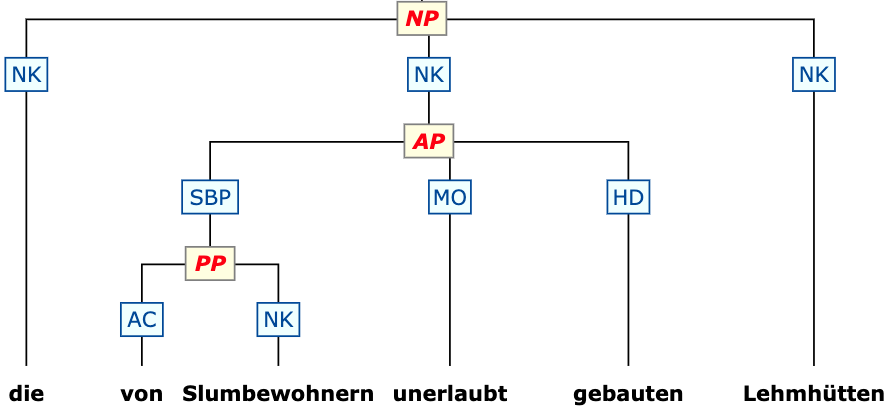
\includegraphics[width=0.75\textwidth]{figures/Treebanks/prePP.png}
    \caption{TIGER tree for (\ref{ex:slum}) (\url{http://hdl.handle.net/11495/D8B8-3970-851A-3@dep101299}) }
    \label{fig:prePP}
\end{figure}

\subsection{Querying with INESS Search}\label{regular} %KDS this subsection does not contain any regular expressions.

% The formulation of
Formulating %hyphenation
well-targeted search expressions presupposes knowledge about the analyses in the treebank.
%It is useful to know something about the representations in the treebank if one wants to formulate useful search expressions.
%In order to be able to formulate useful search expressions, it is necessary to know something about the representations in the treebank.
One way of quickly gaining such knowledge is to use XLE-Web to parse sentences with the kind of grammatical phenomenon one is interested in and to study the analyses.
Suppose that we want to search for passive sentences.
The Norwegian passive sentence in (\ref{ex:skapt-av-gud}) gets the analysis in \figref{fig:skapt-av-gud} when parsed in XLE-Web.

\ea Norwegian\\
\gll Verden ble skapt av Gud.\\  
     {world.\DEF.\SG} was created by God\\ 
\glt `The world was created by God.'
\label{ex:skapt-av-gud}
\z

\begin{figure}
    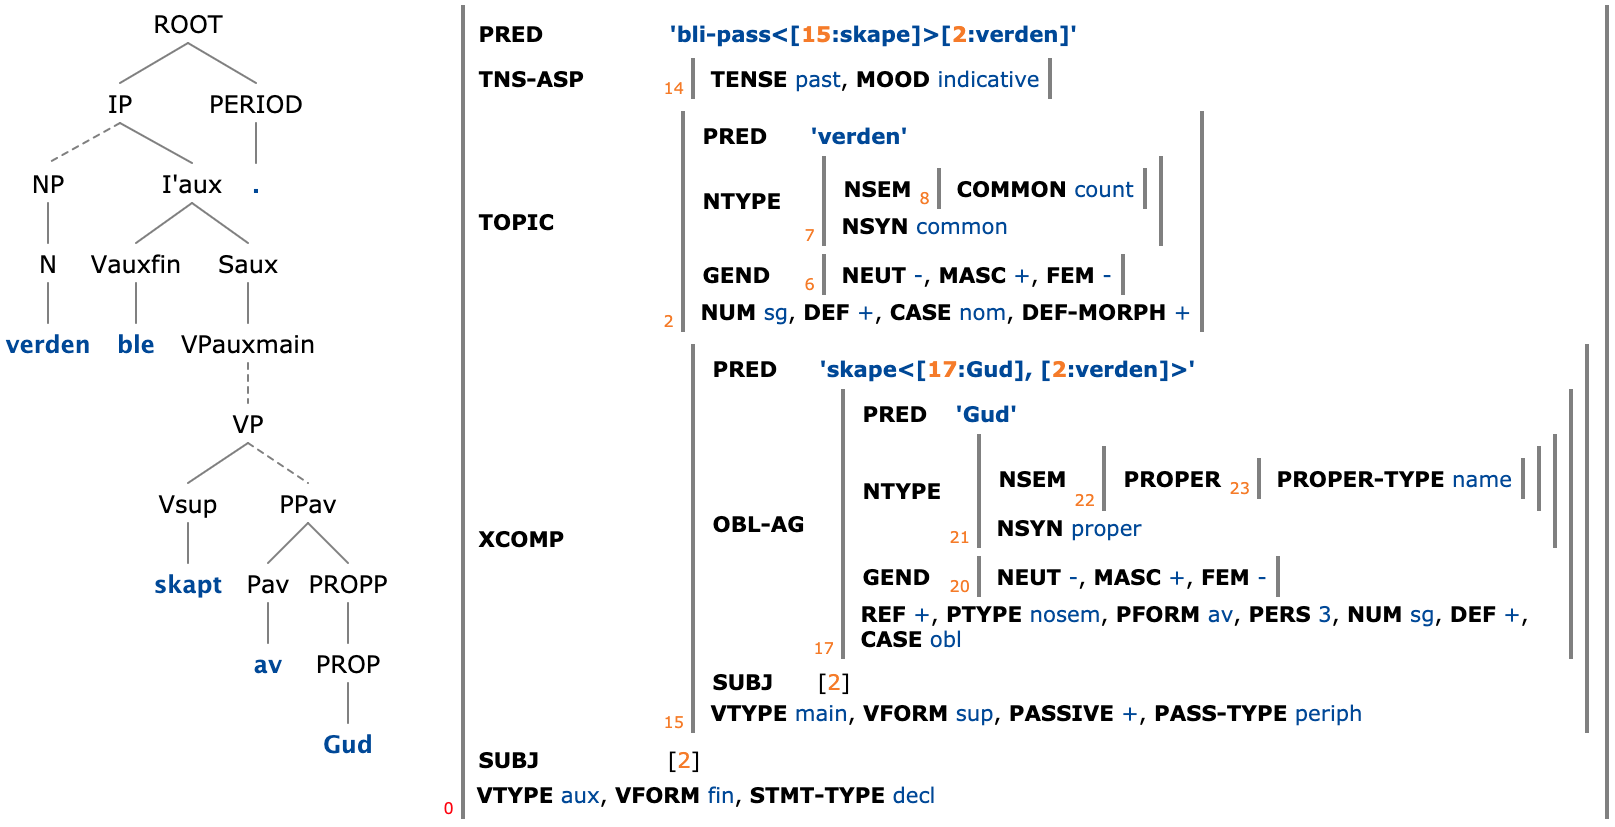
\includegraphics[width=\textwidth]{figures/Treebanks/skapt-av-gud2.png}
    \caption{C- and f-structures from XLE-Web for the passive sentence in (\ref{ex:skapt-av-gud})  }
    \label{fig:skapt-av-gud}
\end{figure}

Examining the f-structure shows that the verb \textit{skape} `create' is the head of the \textsc{xcomp}.
It is a two-place predicate, with the \textsc{pred} of the \textsc{obl-ag}, \textit{Gud} `God', as its first argument, the agent.
The \textsc{xcomp} also has an attribute-value pair `\textsc{passive} +'.
A simple search expression for passives with agent phrases can thus be formulated using these f-structure characteristics, as shown in (\ref{ex:regexp-1}).
%This expression may be read: ``There is an f-structure $\#x$ which has an attribute \textsc{passive} with the value `\textsc +' (bound to $\#y$), and this same f-structure $\#x$ also has an attribute \textsc{obl-ag}.''

%\ea
%\label{ex:regexp-1} %\footnotesize
%\begin{verbatim}
%#x_ >PASSIVE & #x_ >OBL-AG
%\end{verbatim}
%\z

\ea
\label{ex:regexp-1} %\footnotesize
\texttt{\#x >PASSIVE \#y:\textquotesingle+\textquotesingle\ \& \#x >OBL-AG}
%\begin{verbatim}
%#x >PASSIVE #y:'+' & #x >OBL-AG
%\end{verbatim}
\z

This expression may be read: ``There is an f-structure $\#x$ which has an attribute \textsc{passive} with the value `\textsc +' (bound to $\#y$), and this same f-structure $\#x$ also has an attribute \textsc{obl-ag}.''

The negation operator in INESS Search allows users to restrict searches with respect to properties that sentences should \textit{not} have.
The search expression in (\ref{ex:regexp-2}), where the exclamation point is the negation operator, searches for passives \textit{without} agent phrases.
The sentence in (\ref{ex:skapt-no-ag}) is one of those found by this expression; its c- and f-structures are shown in \figref{fig:skapt-no-ag}.
The f-structure nodes that are named with explicit variables in the search expression are marked in red in the search result.
In the f-structure we note that the \textsc{xcomp} does not have an \textsc{obl-ag}, and that the first argument of the main \textsc{pred} is `\textsc{null}'.

\ea
\label{ex:regexp-2} %\footnotesize
\texttt{\#x >PASSIVE \#y:\textquotesingle+\textquotesingle\ \& \#x !>OBL-AG}
%\begin{verbatim}
%#x >PASSIVE #y:'+' & #x !>OBL-AG
%\end{verbatim}
\z

\ea Norwegian  \\
\gll Hvordan er verden skapt?\\  
     how is {world.\DEF.\SG} created\\ 
\glt `How was the world created?'
\label{ex:skapt-no-ag}
\z

\begin{figure}
    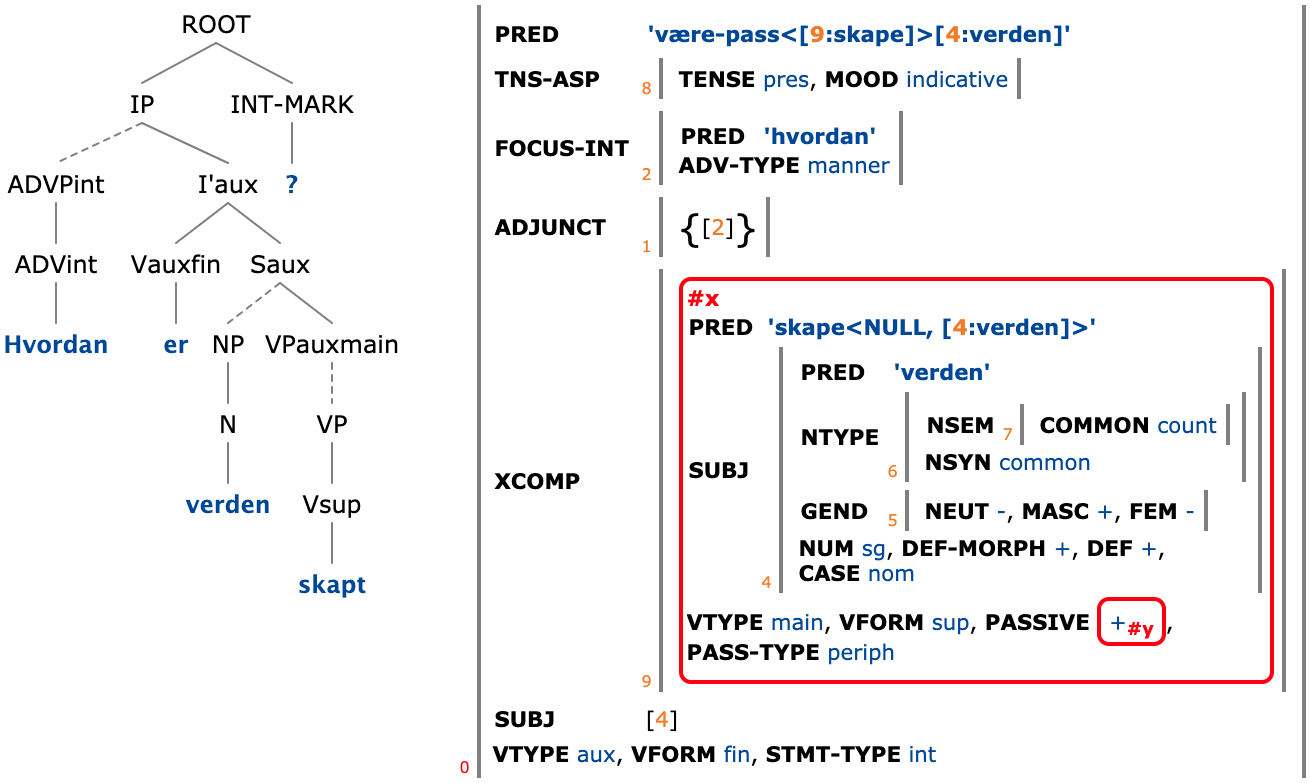
\includegraphics[width=\textwidth]{figures/Treebanks/skapt-no-ag-2.png}
    \caption{C- and f-structures for the passive sentence in (\ref{ex:skapt-no-ag}) (\url{http://hdl.handle.net/11495/D8B8-3970-851A-3@lfg6174124})}
    \label{fig:skapt-no-ag}
\end{figure}



\subsection{An example-based introduction}

For some researchers, INESS Search can be difficult to use, even with the simplifications that have been introduced.
To assist users of NorGramBank in formulating search expressions, an example-based introduction to the search system has been written.\footnote{This introduction, in Norwegian, is part of the INESS documentation: \url{https://clarino.uib.no/iness/page?page-id=norgram-soek\#innledning}.}
It is based on the Norwegian reference grammar \textit{Norsk referansegrammatikk} \citep{Faarlund97nrg} and the chapters and examples therein.
Most researchers in Norwegian syntax will be familiar with the rather theory-neutral analyses in this book, and the goal is to provide them with LFG analyses of the constructions that are of interest, including the page numbers in the book where the constructions are treated.
For each construction, the example-based documentation provides an LFG analysis of one sentence together with a commentary explaining the analysis.
A search expression that will find the construction is provided, along with both a paraphrase and a lengthier prose explanation of the expression.
Finally a list of a few matching sentences is presented.

A construction type that is difficult to search for without a treebank is relative clauses without complementizers. %KDS
It would not be straightforward to find these in corpora which are not syntactically annotated, so this is a good illustration of the added value of treebanks. %KDS
The search expression for relatives without complementizers is given in (\ref{ex:regexp-3}).

\ea
\label{ex:regexp-3}
\texttt{\#x >(ADJUNCT \$) \#f >TOPIC-REL \#g \\
\& \#f >OBJ \#g \& \#f >CLAUSE-TYPE \textquotesingle rel\textquotesingle \\
\& !(\#f >COMP-FORM) \\
\& !(\#x >PRON-TYPE \textquotesingle free\textquotesingle)}
%\begin{verbatim}
%#x_ >(ADJUNCT $) #f_ >TOPIC-REL #g_
%& #f_ >OBJ #g_ & #f_ >CLAUSE-TYPE 'rel'
%& !(#f_ >COMP-FORM)
%& !(#x_ >PRON-TYPE 'free')
%\end{verbatim}
\z

This search expression may be read: ``An f-structure $\#x$ has an attribute \textsc{adjunct} with a value that includes an f-structure $\#f$; furthermore, $\#f$ has an attribute \textsc{topic-rel} with the value $\#g$, and an attribute \OBJ with the same value $\#g$; $\#f$ also has an attribute \textsc{clause-type} with the value `rel' and does not have an attribute \textsc{comp-form}; the f-structure $\#x$ does not have an attribute \textsc{pron-type} with the value `free' (the last specification ensures that free relatives will not be found).''
An example sentence found by this expression in NorGramBank is given in (\ref{ex:alt}), where the boldfaced relative clause \textit{jeg så} lacks a complementizer. %KDS

\ea Norwegian\\
\gll Alt \textbf{jeg} \textbf{så} var frontlykt-ene.\\  
     all I saw was {headlight-\DEF.\PL}\\ 
\glt `All I saw was the headlights.'
\label{ex:alt}
\z

\subsection{Search with templates}\label{templates}

%For some users, INESS Search can be difficult to use, even with the simplifications that have been introduced.
A further simplification in INESS Search is the implementation of search templates, which abbreviate complete parameterized search expressions.
%Therefore, search templates have been implemented.
For the Norwegian treebank NorGramBank, a number of such templates have been provided, primarily for the benefit of lexicographers.\footnote{Documentation in Norwegian:
\url{https://clarino.uib.no/iness/documentation/INESS-Sketch-veiledning-2020.pdf}}
Templates obviate the need for understanding an often complicated search expression, since users can choose one on the basis of a description of its intention, but they can examine the whole expression if desired.
Templates are parameterized in the sense that the user can fill in values for one or more parameters, such as word or lemma forms, predicates, or grammatical features.
%These values then take the place of the parameters in the search expression, and off you go.

Suppose you want to find out how common nominal complement clauses with and without complementizers are after certain verbs.
The template shown in \figref{fig:fortelle}, named \textit{AT-verbwithandwithout(@verb)}, may be used for this purpose.
The user fills in the verb, in this case \textit{fortelle} `tell, relate', and clicks on \textit{Run query}.
The results of the search are presented in a table, sorted according to whether they include the complementizer or not.
We see that the vast majority of occurrences of complement clauses with this verb, 21,465 (97.5\%), do have complementizers.

\begin{figure}
    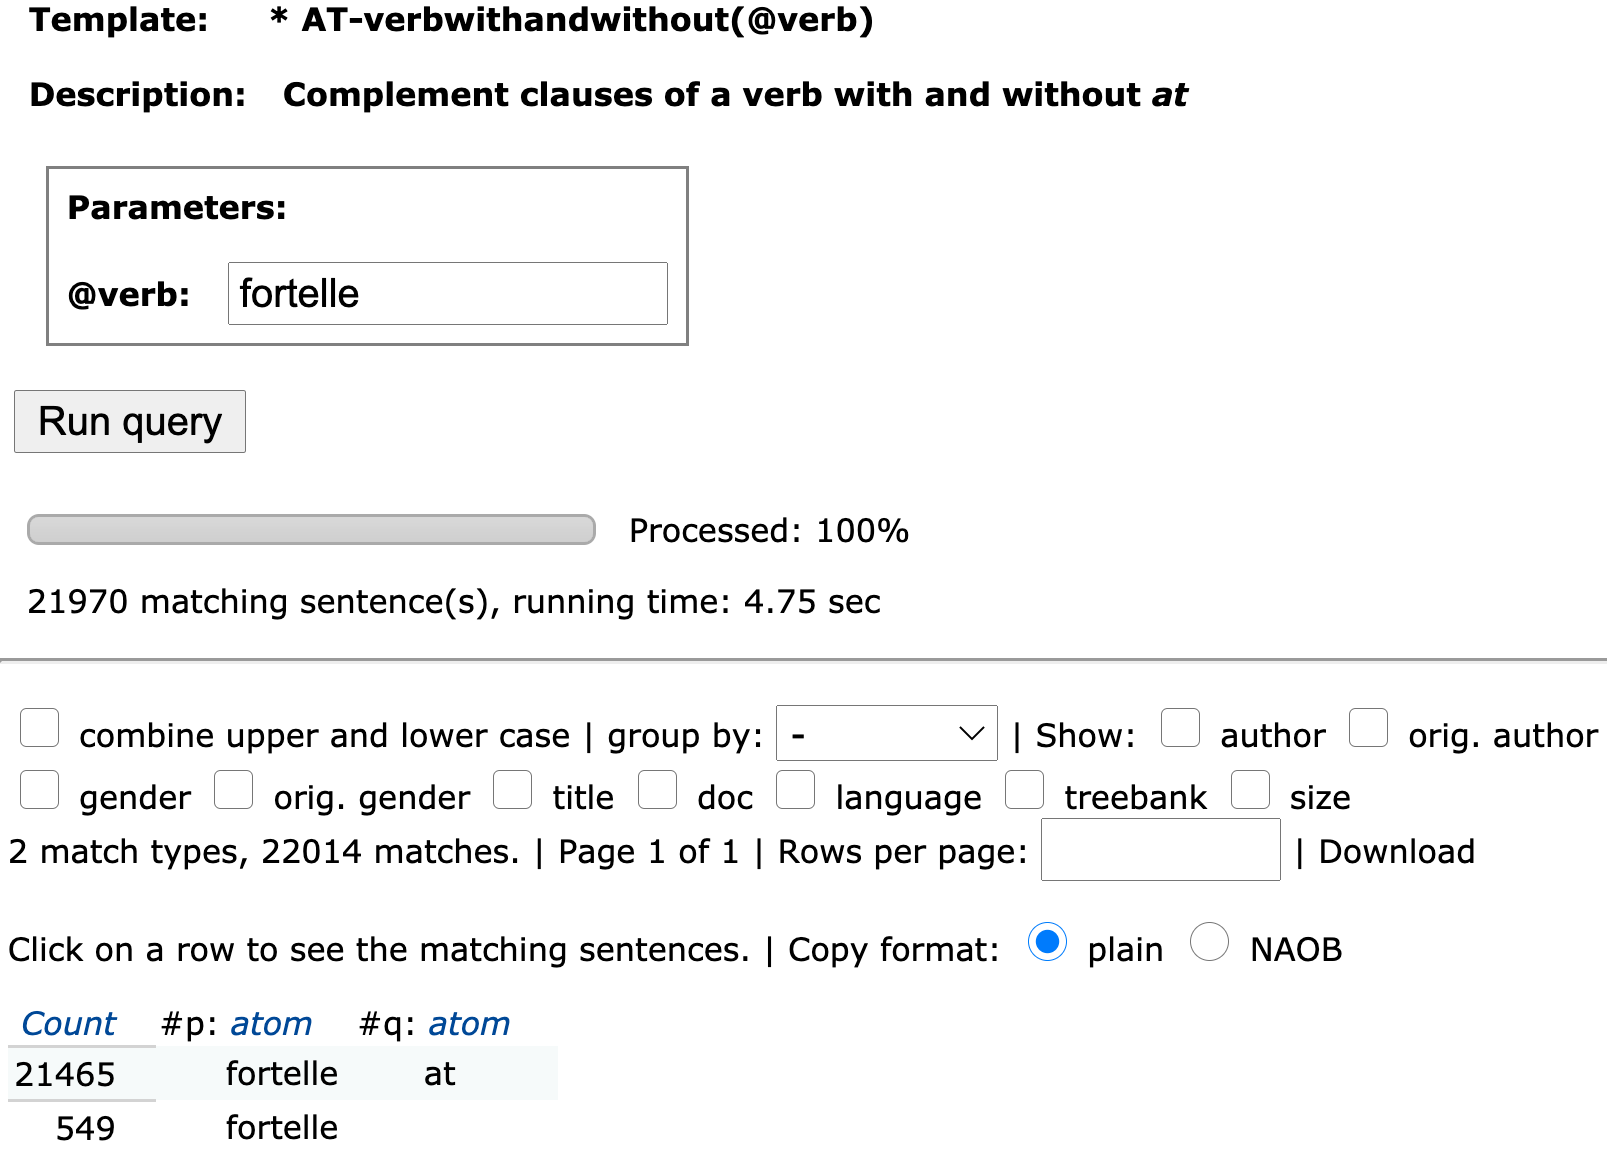
\includegraphics[width=\textwidth]{figures/Treebanks/fortelle.png}
    \caption{Template for nominal clause search with and without complementizer for the verb \textit{fortelle} `tell, relate'}
    \label{fig:fortelle}
\end{figure}

This can be compared with the results for the verb \textit{tro} `think, be of the opinion', shown in \figref{fig:tro}.
For this verb the proportion of uses with the complementizer is only 33.8\%.
In this screenshot the user has clicked on the first row in the table, showing the number of occurrences for the verb without the complementizer (66,258).
This brings up a list over all the sentences with this pattern.
Here the user has clicked twice on \textit{Next} in order to come to page 3; there are so many hits that the list consists of 3,313 pages.
When the user mouses over a sentence, a simplified f-structure is displayed to the right of the list.
Clicking on a sentence brings the user to the \emph{Sentence} page where the c-structure and the full f-structure are displayed.
By default the quite complicated search expression which is used in this template is hidden, as in \figref{fig:fortelle}.
In \figref{fig:tro}, the user has clicked on the template name, bringing up the expansion with the search expression.
In this figure a more detailed prose description is also displayed, obtained by clicking on the boldfaced, more compact, part of the description.
%Clicking on the boldfaced part of the description brings up the more detailed prose description displayed here.


\begin{figure}
    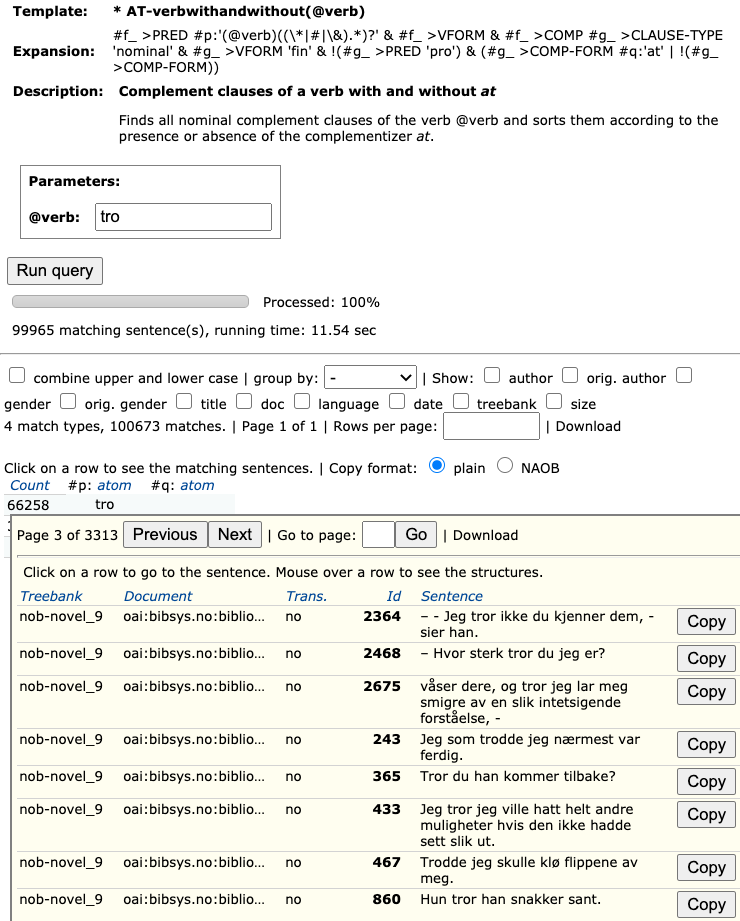
\includegraphics[width=\textwidth]{figures/Treebanks/tro-new.png}
    \caption{Template for nominal clause search with and without complementizer for the verb \textit{tro} `think, be of the opinion'}
    \label{fig:tro}
\end{figure}

\citet{RausetEtAl:Words} provide concrete examples of the use of template search in NorGramBank for various dictionary projects in Norway.
The lexicographers use templates to examine both the usage and frequency of words.
The most common valency frames for verbs, as well as the most common prepositions and/or particles that they occur with, are examined by using the template \textit{V-argframes(@V)}; this template also provides evidence about whether the verbs occur reflexively.
The templates \textit{ADJ-attrib-or-nominal(@ADJ)}  and \textit{V-attr-or-pred-ptc(@V)} provide evidence of the nominal and adjectival use of participles, which is sometimes the basis for the creation of separate entries for derived adjectives.

\newpage
Targeted queries that provide evidence for colligations are useful when treating high-frequency words with many senses.
The template \textit{N-argofverbs(@N)} provides a list sorted by frequency of the verbs that occur with a certain noun as their first or second argument.
Such results help lexicographers determine whether the sense distinctions made in older versions of the dictionaries are still reasonable, or whether there should be changes made by adding or removing distinctions, or for instance by promoting a sense that is now more common than previously.

An example of a word which was missing a sense is the reflexive verb \textit{utmerke seg} `distinguish oneself', which was defined as having only a positive connotation.
The lexicographers, however, did not believe this to be accurate.
The template \textit{V-prepobj(@V,@P)} was used to examine which words occur as objects of the prepositions \textit{med} `with' and \textit{ved} `by'.
The search results showed several occurrences of the noun \textit{mangel} `lack' as the object of \textit{ved}; one of these examples is given in (\ref{ex:mangel}).
This and similar searches provided empirical support for the establishment of a new subsense of the verb with a negative connotation.

\ea Norwegian (\url{http://hdl.handle.net/11495/D8B8-3970-851A-3@lfg14979442}) \\
\gll Han vil ... utmerke seg med mangel på konsistens i sine handlingsvalg ...\\  
     he will {} distinguish \textsc{refl} with lack of consistency in his {action.choice}\\ 
\glt `He will ... distinguish himself with lack of consistency in his choice of actions ... '
\label{ex:mangel}
\z

\subsection{Comparison of search in LFG and dependency treebanks}\label{comparison}

Dependency treebanks are the most widely used type of treebanks, notably
%through
via the Universal Dependencies (UD) initiative.\footnote{\url{https://universaldependencies.org}}
The UD treebanks are grounded in dependency grammar, which assigns dependency relations between words, and does not analyze phrases and constituency relations \citep{Tesniere1959}.
An important early dependency treebank was the Prague Dependency Treebank \citep{Hajic01}.
Among the treebanks provided by INESS, dependency treebanks are the most numerous (250), with the UD treebanks accounting for most of these (200).
The latest version in INESS at the time of writing is 2.8. INESS also keeps earlier versions, making it possible to track progress between versions.

The LFG and UD analyses of the sentence in (\ref{ex:lykkelig}) are shown in \figsref{fig:happy-LFG}{fig:happy-UD-morph}.
For both treebanks, information about lemma, part of speech and morphological features may be displayed (by clicking on the word for the dependency treebank, or by clicking on the preterminal node for the LFG treebank).
The c-structure in \figref{fig:happy-LFG} shows the hierarchical phrase structure of the sentence, labeled with a rich inventory of syntactic categories.
The corresponding f-structure encodes syntactic functions, grammatical features, and predicate--argument relations, as represented in the semantic forms of the verbs.
The dependency structure in \figref{fig:happy-UD-morph} is shallower and less detailed than the LFG structure. %KDS
Dependencies between words are shown by labeled arrows that go from a word to its dependents.


\ea Norwegian\\
\gll Han hadde aldri vært lykkeligere.\\  
     he had never been happier\\ 
\glt `He had never been happier.'
\label{ex:lykkelig}
\z

\begin{figure}
    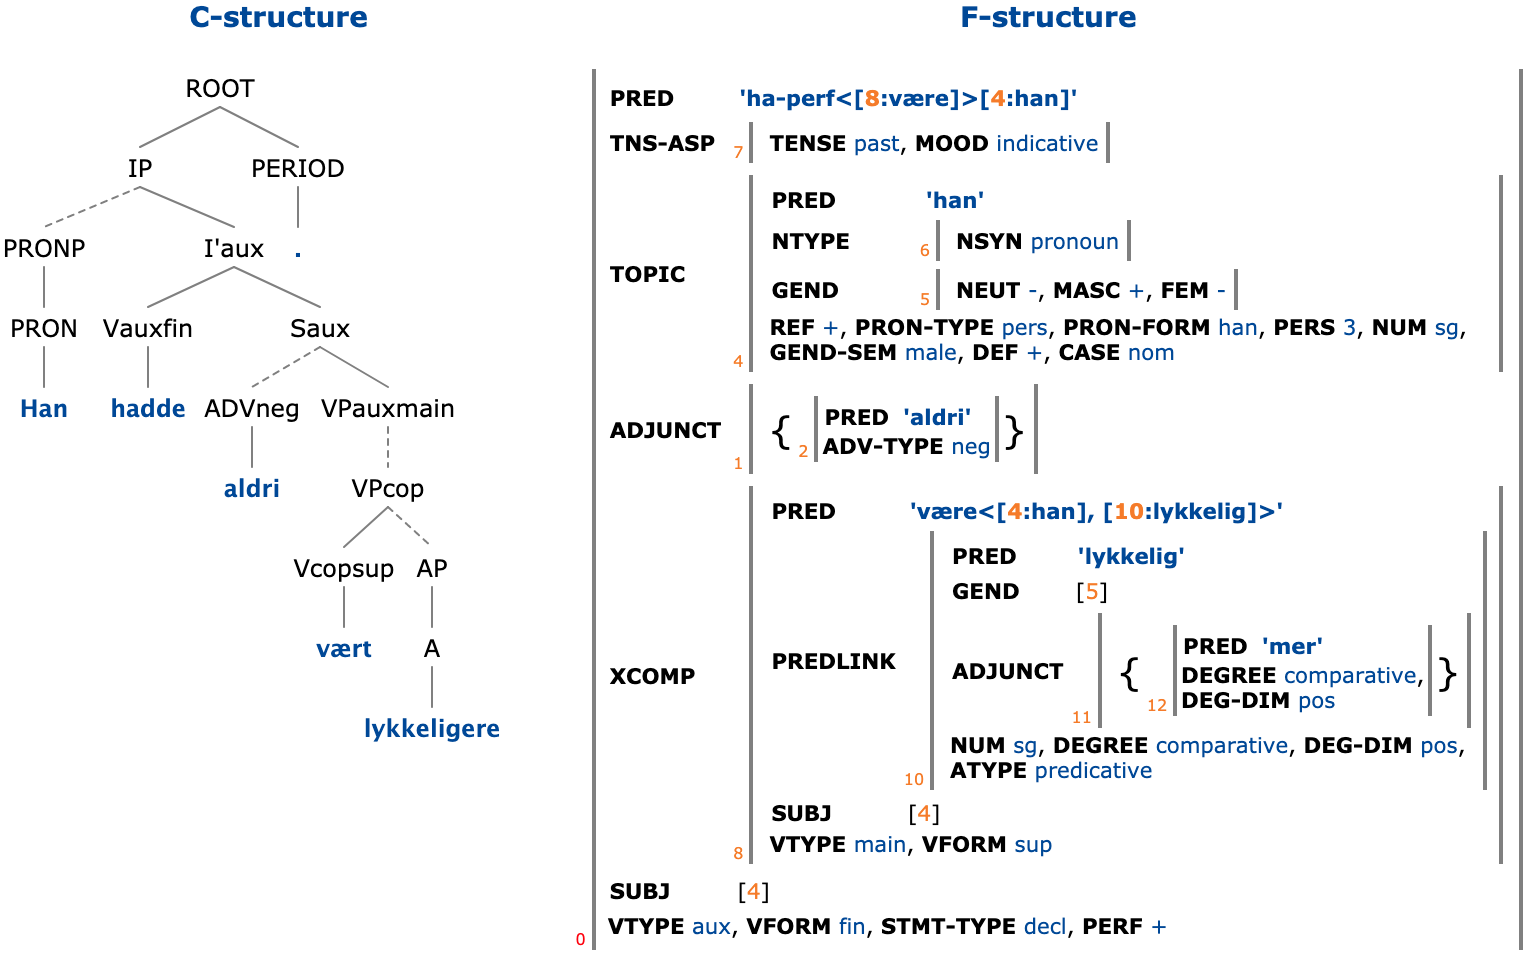
\includegraphics[width=\textwidth]{figures/Treebanks/happy-LFG.png}
    \caption{LFG analysis of the sentence in (\ref{ex:lykkelig}) (\url{http://hdl.handle.net/11495/D8B8-3970-851A-3@lfg4292653}) }
    \label{fig:happy-LFG}
\end{figure}

\begin{figure}
    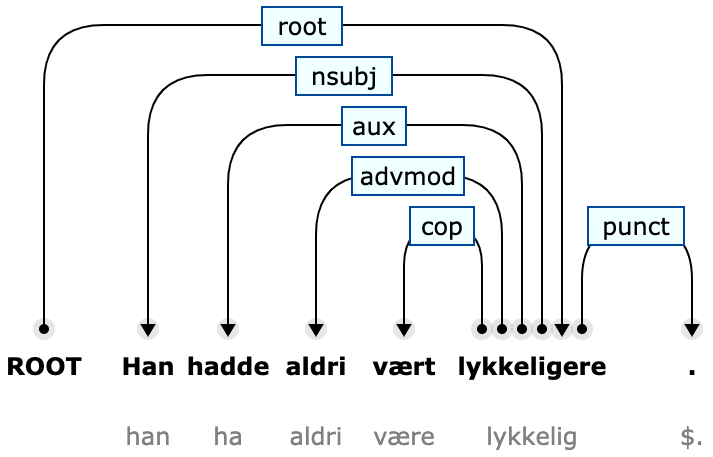
\includegraphics[width=0.5\textwidth]{figures/Treebanks/happy-UD.png}
    \caption{UD analysis of the sentence in (\ref{ex:lykkelig}) (\url{http://hdl.handle.net/11495/D8B8-3970-851A-3@dep8965528}) }
    \label{fig:happy-UD-morph}
\end{figure}

The deeper analysis in an LFG treebank improves the search possibilities as compared with a dependency treebank.
\citet{Rosen20creating} compares search in the UD version of the Norwegian Dependency Treebank with the same texts in NorGramBank.
The example given there is searching for the first argument of verbs.
This may be done straightforwardly in an LFG treebank, but it is much more difficult in a dependency treebank since predicate--argument structure is not encoded there.
The first argument of a verb can be the subject of an active verb or of a predicative present participle, the agent phrase of a passive verb, or the head of an attributive present participle.
And since the UD guidelines allow for several ways of annotating some of these possibilities, creating a search expression to capture them is extremely complicated.
For more detail on this comparison, see \citet{Rosen20creating}.



%\ea
%\gll Drzewo zostało ścięte wczoraj.\\  
%     tree was cut yesterday\\ 
%\glt `The tree was cut down yesterday.'
%\z

%\begin{figure}
%    \centering
%    \includegraphics[width=\textwidth]{Polish-cf}
%    \caption{C- and f-structures for Polish}
%    \label{fig:Polish-cf}
%\end{figure}


%\eal
%\label{query-overlate} \small
%\begin{verbatim}
%#f_ >PRED #a:'overlate' & ((#f_ >(ARG1 NTYPE NSYN) #arg1 
%| #f_ >(ARG1 VFORM) #arg1 | !(#f_ >ARG1)) & !(#f_ >ARG2) 
%| (#f_ >(ARG1 NTYPE NSYN) #arg1 | #f_ >(ARG1 VFORM) #arg1 %
%| !(#f_ >ARG1)) & (#f_ >(ARG2 NTYPE NSYN) #arg2 
%| #f_ >(ARG2 VFORM) #arg2) & !(#f_ >ARG3)) 
%| (#f_ >(ARG1 NTYPE NSYN) #arg1 | #f_ >(ARG1 VFORM) #arg1 %
%| !(#f_ >ARG1)) & (#f_ >(ARG2 NTYPE NSYN) #arg2 
%| #f_ >(ARG2 VFORM) #arg2) & (#f_ >(ARG3 NTYPE NSYN) %#arg3
%| #f_ >(ARG3 VFORM) #arg3) & #f_ >VFORM
%\end{verbatim}
%\zl

\section{Conversion between LFG treebanks and other treebanks}\label{depbanks}

%\citet{Abeille03b}

%\citet{Treebankwhitepaper}

Besides pure parsebanking with a grammar, other approaches have been used to construct treebanks by converting between formalisms or by enriching treebanks with additional information.
The Universal Dependencies initiative is in some ways similar to ParGram in that both approaches aim at assigning common annotations to comparable items and structures across languages.
%Dependency grammar assigns dependency relations between words, and notably does not analyze phrases and constituency relations.

Since dependency relations may be labeled as grammatical functions such as subject and object, dependency structures have a resemblance to f-structures in LFG.
%There have been various efforts to create dependency treebanks from LFG treebanks.
The PARC 700 Dependency Bank is a treebank in dependency format based on the English LFG grammar developed at PARC \citep{Parc700}.
The corpus was created only to make a dependency bank.
LFG analyses were transformed to dependency graphs, but no LFG treebank per se was created.

The TIGER corpus, mentioned in \sectref{tiger}, utilized the large-scale German LFG grammar of the ParGram project for the semiautomatic creation of TIGER treebank annotations.
The grammar was used for full parsing, followed by semi-automatic disambiguation and automatic transfer into the treebank format \citep{zinsmeisteretal02}.
The hybrid representation structure of TIGER, combining constituent analysis and functional dependencies, benefited from information in the c-structures and f-structures provided by the LFG grammar.

Conversely, an LFG treebank may be created by enriching phrase-structure oriented treebank resources with functional structures, as suggested by \citet{Frank03} and \citet{Cahill04thesis}.
%Although these authors have described algorithms for doing this, no substantial treebanks have actually been created with this methodology.
For more on grammar induction, see \citetv{chapters/GrammarInduction}.

\citet{forst-2003-treebank} describes a method for converting the TIGER treebank to a testsuite for the German LFG ParGram grammar.
The conversion utilizes the machine translation transfer system in XLE.

Recently, detailed algorithms for the conversion from LFG analyses to dependency structures were proposed by \citet{Meurer17LFG} and \citet{prz:pat:19:lre}.
While the latter follow the more standard assumption that f-structures provide a good basis for developing dependency trees, the former takes c-struc\-tures as the starting point, but combines this with information from f-structures.


%Visualization in INESS: vis. the effects of discriminants on packed structures, vis. of search results, interactive vis. of LFG structures mouseover, accross projections etc.

%NorGramBank evaluation, see NorGramBank paper (Dyvik et al. LREC 2016): grammar coverage, annotator and disambiguator precision and types of annotator disagreement

\section{Conclusion}\label{concl}

This chapter has provided an introduction to LFG treebanks, illustrated throughout with the tools and visualizations of the INESS treebanking infrastructure.
The process of developing an LFG grammar in tandem with a treebank through incremental parsebanking has been described.
Both large and small LFG parsebanks for a number of languages have been presented.
Several different methods for searching LFG treebanks with INESS Search have been explained: users can write search expressions themselves with the aid of XLE-Web and the INESS Search documentation; they can find search expressions for the phenomena they are interested in by consulting the example-based search documentation; and they can use search templates that only require filling in one or more search items.
LFG treebanks have been compared with other treebanks, and it has been shown that the more detailed and sophisticated annotation in LFG treebanks provides richer opportunities for research than simpler annotations.

While INESS has already been developed over more than a decade, the system, and especially its interface, will continue to evolve. %KDS
Consequently, future interactions may be slightly different from the interactions and screen displays shown in this chapter. %KDS

Although LFG treebanks are certainly valuable resources for research and development, building an LFG treebank is a time-consuming and expensive undertaking, especially for a language for which no large-coverage LFG grammar and lexicon yet exist. %KDS
However, the task is made somewhat easier with the help of the LFG Parsebanker as described above, and INESS is open to making more treebanks accessible for research and development. %KDS


%From VISLR article:

%A potentially useful addition would be the ability to shrink large structures with zooming so that the user can mouse over with an intuitive virtual mag- nifying glass in order to zoom into parts. Another addition might be the option to lock highlighting which is now only shown during mouse over. Also, it may be useful to have interactions (e.g. highlighting) between words in a linear version of the sentence and their corresponding nodes in syntactic structures. Finally, the construction of queries would benefit from some interactive support, e.g. through feedback on the query as it is being written, by means of color coding or otherwise.


%\section*{Abbreviations}
\section*{Acknowledgments}

I thank Koenraad De Smedt, Stefanie Dipper, Helge Dyvik, Jonas Kuhn, Paul Meurer, Agnieszka Patejuk, Heike Zinsmeister and three anonymous reviewers for helpful comments and suggestions.
Thanks are also due to Mary Dalrymple for all of her help and her boundless patience.
  
\sloppy
\printbibliography[heading=subbibliography,notkeyword=this]
\end{document}
